\documentclass{article}\usepackage[]{graphicx}\usepackage[]{color}
% maxwidth is the original width if it is less than linewidth
% otherwise use linewidth (to make sure the graphics do not exceed the margin)
\makeatletter
\def\maxwidth{ %
  \ifdim\Gin@nat@width>\linewidth
    \linewidth
  \else
    \Gin@nat@width
  \fi
}
\makeatother

\definecolor{fgcolor}{rgb}{0.345, 0.345, 0.345}
\newcommand{\hlnum}[1]{\textcolor[rgb]{0.686,0.059,0.569}{#1}}%
\newcommand{\hlstr}[1]{\textcolor[rgb]{0.192,0.494,0.8}{#1}}%
\newcommand{\hlcom}[1]{\textcolor[rgb]{0.678,0.584,0.686}{\textit{#1}}}%
\newcommand{\hlopt}[1]{\textcolor[rgb]{0,0,0}{#1}}%
\newcommand{\hlstd}[1]{\textcolor[rgb]{0.345,0.345,0.345}{#1}}%
\newcommand{\hlkwa}[1]{\textcolor[rgb]{0.161,0.373,0.58}{\textbf{#1}}}%
\newcommand{\hlkwb}[1]{\textcolor[rgb]{0.69,0.353,0.396}{#1}}%
\newcommand{\hlkwc}[1]{\textcolor[rgb]{0.333,0.667,0.333}{#1}}%
\newcommand{\hlkwd}[1]{\textcolor[rgb]{0.737,0.353,0.396}{\textbf{#1}}}%
\let\hlipl\hlkwb

\usepackage{framed}
\makeatletter
\newenvironment{kframe}{%
 \def\at@end@of@kframe{}%
 \ifinner\ifhmode%
  \def\at@end@of@kframe{\end{minipage}}%
  \begin{minipage}{\columnwidth}%
 \fi\fi%
 \def\FrameCommand##1{\hskip\@totalleftmargin \hskip-\fboxsep
 \colorbox{shadecolor}{##1}\hskip-\fboxsep
     % There is no \\@totalrightmargin, so:
     \hskip-\linewidth \hskip-\@totalleftmargin \hskip\columnwidth}%
 \MakeFramed {\advance\hsize-\width
   \@totalleftmargin\z@ \linewidth\hsize
   \@setminipage}}%
 {\par\unskip\endMakeFramed%
 \at@end@of@kframe}
\makeatother

\definecolor{shadecolor}{rgb}{.97, .97, .97}
\definecolor{messagecolor}{rgb}{0, 0, 0}
\definecolor{warningcolor}{rgb}{1, 0, 1}
\definecolor{errorcolor}{rgb}{1, 0, 0}
\newenvironment{knitrout}{}{} % an empty environment to be redefined in TeX

\usepackage{alltt}
\usepackage[english]{babel}
\usepackage[T1]{fontenc}
\usepackage[utf8]{inputenc}
\usepackage[margin=1in]{geometry}
\usepackage{enumitem}
\usepackage{amsmath}
\usepackage{mathtools}
\usepackage{amssymb}
\usepackage{physics}
\usepackage{booktabs}
\usepackage{bm}
\usepackage{dirtytalk}
\usepackage{epigraph} 
\usepackage{hyperref}
\usepackage{comment}
\usepackage{graphicx}
\usepackage{wallpaper}
\usepackage{natbib}

\title{Bayesian data analysis – Final project, Part 1}
\author{Kári Rögnvaldsson}
\date{\today}

\newcommand{\solution}{\medskip\par\textbf{Solution: }}
\newcommand{\p}{\text{Pr}}
\newcommand{\Var}[1]{\operatorname{Var}\qty(#1)}
\newcommand{\E}[1]{\operatorname{E}\qty(#1)}
\newcommand{\problem}[1]{\section*{Problem #1}}
\newcommand{\N}{\mathcal{N}}

\setlength{\parindent}{0pt}
\IfFileExists{upquote.sty}{\usepackage{upquote}}{}
\begin{document}

\ThisULCornerWallPaper{1}{front_page/hi_front_page.pdf}
%\ThisLLCornerWallPaper{1}{logo.png}
%\heading{Music genres}
%\begin{adjustbox}{center}
%{\Large Classification and Recommendation}
%\end{adjustbox}


\begin{titlepage}
    \begin{center}
        \vspace*{4cm}
            
        \Huge
        \textbf{Prediction model for the PGA Tour}
            
        \vspace{0.5cm}
        \Large
        A Bayesian method
            
        \vspace{1.5cm}
            
        \large
        Kári Rögnvaldsson (kar26@hi.is) \\
            
        \vfill
            
        Final project in STÆ528M
            
        \vspace{0.8cm}
            
        \large
        Instructor: Birgir Hrafnkelsson \\
        \today
            
        \vspace{1cm}
        
\includegraphics[scale=0.4]{front_page/hi_logo.png}
    \end{center}
\end{titlepage}

\newpage

\section{Introduction}
\epigraph{Competitive golf is played mainly on a five-and-a-half-inch course, the space between your ears.}{\textit{Bobby Jones}}

Golf is a sport played by millions of people around the world. It is a sport circled around competing with yourself to get better every time you play and one needs a very strong mental mindset to be able to succeed. The goal of golf is to put a small golf ball into a hole in as few strokes as possible. A round of golf is traditionally eighteen holes and a professional tournament of golf traditionally consists of four rounds that are played from Thursday thru Sunday. The PGA Tour (Professional Golfers Association) is the largest stage for competitive golf in the world, where elite golfers compete with each other to become the best in the world. Almost every weekend, there is a tournament that takes place on a course somewhere in the world, most often in the United States. In the tournaments, around 120 players bring their best in trying to come out on top.
\medskip\par
There are extremely many factors that make a tournament winner, some of the most important are how the course fits the golfer and the player's physical and mental form. In this project, we aim to model golfer's performance and determine winners and top players in tournaments. More specifically, what is the probability that a given player is the winner of a given tournament? What is the probability that he will place in the top 10, top 25, and what is the probability that is cut out of the tournament after two days (misses the cut)? To answer these questions, we will use a hierarchical linear model based on the player.

\section{Prevoius work}
Some people have been experimenting with golf predictive models, such as \cite{courchene_2018}. The model in this study is inspired by that model, but differs in many respects. Others, like \cite{inproceedings} have experimented with hierarchical models for sports, which is very interesting. A description of the Bayesian hierarchical models used and many other techniques are found in \cite{bda3}

\section{Data}
\subsection{The dataset}
The project consists of a player based dataset. The dataset is obtained from the following website: \url{https://www.advancedsportsanalytics.com/pga-raw-data}. It consists of roughly 33,000 data points for almost 500 players on the PGA Tour from 2015–2021. The most important columns of the data are the following:
\medskip\par
\hspace{4em}\verb$player$: Player's full name

\hspace{4em}\verb$tournament_name$: Name of the tournament that is recorded in the data point.

\hspace{4em}\verb$course$: The name of the course played in the tournament.

\hspace{4em}\verb$date$: Date of the tournament.

\hspace{4em}\verb$pos$: Final position of the player in the tournament.

\hspace{4em}\verb$hole_par$: The par of the course.

\hspace{4em}\verb$strokes$ Number of strokes for the player in the tournament.

\hspace{4em}\verb$made_cut$: A value, either 1 or 0, that indicates if a player made the cut.
\medskip\par 
A ''missed cut'' is when a player does not qualify high enough the first two days of the tournament.
\subsection{Data manipulation}
A player's performance relative to the other players that are competing is of most interest and therefore it is not needed to estimate the total number of strokes for each player. There is a massive difference between courses in difficulty, so we need to account for a course being hard/easy. For each tournament, a statistic that we will here call ''standardized strokes gained'',  is calculated as follows: For every tournament a player plays, the average number of strokes per round is calculated, let us call that $S_{ij}$ where $i$ denotes player $i$ and $j$ denotes tournament $j$, the quantity $SG$ (strokes gained) is calculated
\[SG_{ij} = \frac{S_{ij}-\mu_j}{s_j},\]
where 
\[\mu_j = \frac1n \sum_{k}S_{kj} \quad \text{and}\quad s_j^2 = \frac{1}{n-1}\sum_{k}(S_{kj}-\mu_j)^2,\]
i.e. the $S_{ij}$ terms are normalized to have mean zero and standard deviation 1 over all $i$ for fixed tournament $j$. This quantity is a measure of a player's performance relative to the field and will be used to predict.
\medskip\par 
There is also some time element in a player's performance on the field according to the graph in section 3.3. If we denote the day of of tournament $j$ for player $i$ as $t^\ast_{ij}$, where $t^\ast_{ij}$ is the number of days since the first tournament in the dataset was played, we let
\begin{align*}
    t_{ij} = 2\frac{t_{ij}^{\ast}-t_0}{t^{\ast}_{\text{max}}},
\end{align*}
where $t^{\ast}_\text{max}$ is the latest date in the data and $t_0$ is the median value of $t^\ast$. The quantity $t_{ij}^{\ast}$ has therefore been scaled such that $t_{ij} \in [-1;1]$.

\subsection{Data exploration}
When $SG_{ij}$ is plotted for a player as a function of time, we obtain figures like Figures \ref{fig:spieth_progress}. Figure \ref{fig:spieth_progress} shows the progress for Jordan Spieth, a top class golfer, along with a smooth fit of the data to visualize the trend more. We see that there is a time trend in the data and Jordan Spieth is extremely interesting because of the dip in the trend. He was the top ranked golfer in the world in 2016, then he underperformed from 2018-2020 and in the year 2021, he has performed better again. This is apparent in the smooth curve fitted to the data. That curve is what we want to model. If we look at empirical density of the $SG$ variable on a player basis, we note a left tail in the data (see Figures \ref{fig:thomas_empirical_density}, \ref{fig:spieth_empirical_density}, \ref{fig:rahm_empirical_density} and \ref{fig:dechambeau_empirical_density}). This might be because golf is a sport that is extremely hard to play at a high level and very easy to play bad. Therefore, very bad scores are more likely than very good scores and thus, the distributions becomes left tailed.

\begin{figure}[h]
    \centering
    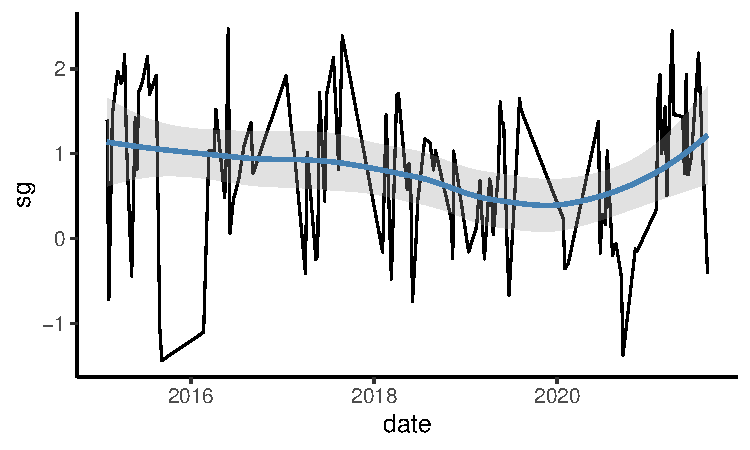
\includegraphics[width=4in]{Figures/progress_trend_spieth.pdf}
    \caption{Form trend of Jordan Spieth}
    \label{fig:spieth_progress}
\end{figure}

\begin{figure}[h]
\begin{minipage}{0.475\textwidth}
    \centering
    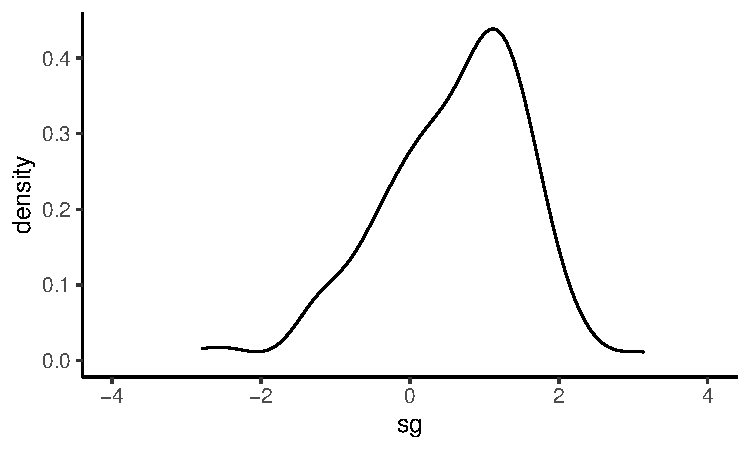
\includegraphics[width=1\textwidth]{Figures/empirical_density_thomas.pdf}
    \caption{Empirical density for standardized strokes gained for Justin Thomas}
    \label{fig:thomas_empirical_density}
\end{minipage}
\hspace{0.05\textwidth}
\begin{minipage}{0.475\textwidth}
    \centering
    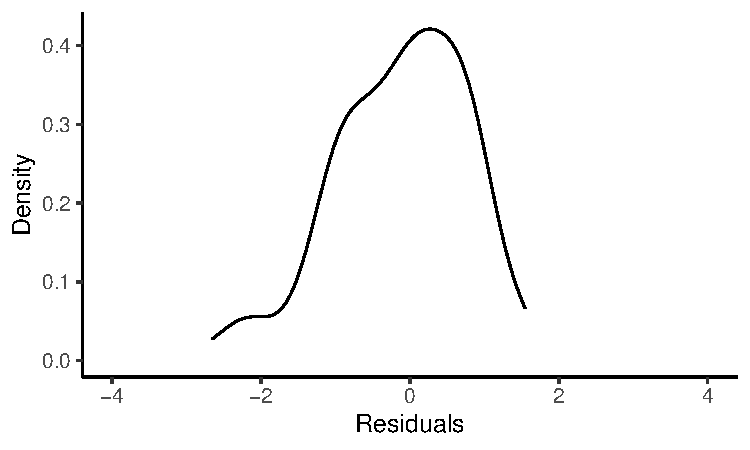
\includegraphics[width=1\textwidth]{Figures/empirical_density_spieth.pdf}
    \caption{Empirical density for standardized strokes gained for Jordan Spieth}
    \label{fig:spieth_empirical_density}
\end{minipage}
\end{figure}
%
\begin{figure}[h]
\begin{minipage}{0.475\textwidth}
    \centering
    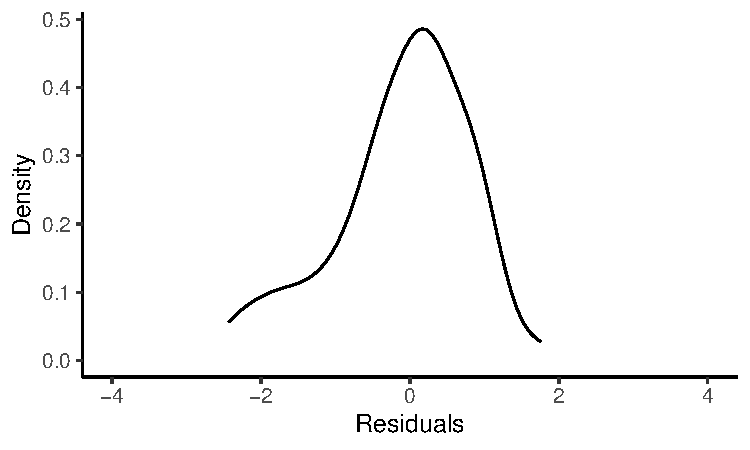
\includegraphics[width=1\textwidth]{Figures/rahm_empirical_density.pdf}
    \caption{Empirical density for standardized strokes gained for Jon Rahm}
    \label{fig:rahm_empirical_density}
\end{minipage}
\hspace{0.05\textwidth}
\begin{minipage}{0.475\textwidth}
    \centering
    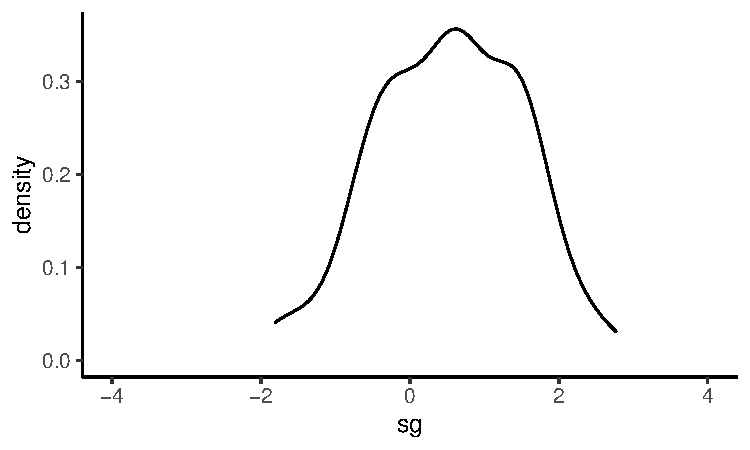
\includegraphics[width=1\textwidth]{Figures/empirical_density_dechambeau.pdf}
    \caption{Empirical density for standardized strokes gained for Bryson DeChambeau}
    \label{fig:dechambeau_empirical_density}
\end{minipage}
\end{figure}
\newpage

\subsection{Corrupt data}
Some of the tournaments in the date were not fully recorded. From some, it was quite obvious that there were players that played in the tournament that were not in the data, since all or almost all the players in the data made the cut in a specific tournament, which is not realistic. Therefore, the tournaments with over $80\%$ of the players making the cut were removed. This choice was arbitrary, but it is unrealistic that more than $80\%$ of the players make the cut. If too many players in a tournament in the data make the cut it is highly likely that the data does not show the full competition and we thus do not get a correct image of the relative performance. It is usually around the first 70 players that make the cut after two days, of around 120 total players, which makes 58\%.

\section{Statistical models}
In this section, we will present the model that is used in the study.

\subsection{Model introduction}
As stated in the data section, it is aimed at to predict the number of standardized shots gained of the players competing in a given tournament. Since the data is left-tailed, we model the $SG$ variable as a Mirror-Gumbel variable. To model the time, we introduce a 3rd degree polynomial to describe the evolution of the player in time. Shots gained for player $i$ in tournament $j$ therefore becomes
\begin{align*}
    SG_{ij} \sim \text{Mirror-Gumbel}(\alpha_{0,i} + \alpha_{1,i}t + \alpha_{2,i}t^2 + \alpha_{3,i}t^3, e^{\beta_i})
\end{align*}
where $\alpha_{k,i}$ is parameter $k$ in the 3rd degree polynomial for the expected value of $SG$ for player $i$ and $e^{\beta_i}$ is the dispersion parameter of the Mirror-Gumbel distribution for player $i$. We need to use the Mirror-Gumbe since the standard Gumbel distribution is right tailed and this dataset is left tailed. Note that the PDF for the mirrored gumbel distribution is
\begin{align*}
    p(y|\mu,\beta) = \frac1\beta\exp(-(z+\exp(-z)))
\end{align*}
where $z\coloneqq\frac{\mu-y}{\beta}$. The CDF becomes
\begin{align*}
    F(y|\mu,\beta) = e^{e^{-z}}
\end{align*}
and the inverse CDF (for sampling from the distribution with inverse CDF methods) becomes
\begin{align*}
    F^{[-1]}(x|\mu,\beta) = \mu + \beta\log(-\log{x}).
\end{align*}
Note that the regular Gumbel distribution is the same but with $z\coloneqq\frac{y-\mu}{\beta}$.
\medskip\par 
We have 5 variables for each of the players. Since we expect all these parameters to be similarily distributed, we assume
\begin{align*}
    &\alpha_{k,i} \sim \N(\mu_{\alpha_k}, \sigma_{\alpha_k}^2), \\
    &\beta \sim N(\mu_\beta, \sigma_\beta^2)
\end{align*}
where we assign the weakly informative hyperpriors
\begin{align*}
    &\mu_{\alpha_k} \sim \N(0,5^2), \\
    &\mu_\beta \sim \N(0,5^2), \\
    &\sigma^2_{\alpha_i} \sim \text{Inv–}\chi^2(1, 5^2), \\
    &\sigma_\beta^2 \sim \text{Inv–}\chi^2(1, 5^2).
\end{align*}
The model hierarchy becomes as follows:
\medskip\par 
\emph{Hyperparameters:}
\begin{align*}
     &\mu_{\alpha_k} \sim \N(0,5^2), \\
    &\mu_\beta \sim \N(0,5^2), \\
    &\sigma^2_{\alpha_i} \sim \text{Inv–}\chi^2(1, 5^2), \\
    &\sigma_\beta^2 \sim \text{Inv–}\chi^2(1, 5^2).
\end{align*}
\smallskip\par 
\emph{Latent level:}
\begin{align*}
    &\alpha_k|\mu_{\alpha_k}, \sigma_{\alpha_k} \sim \N(\mu_{\alpha_k}, \sigma_{\alpha_k}^2) \\
    &\beta_i|\mu_\beta, \sigma_\beta \sim \N(\mu_\beta,\sigma_\beta^2)
\end{align*}
\smallskip\par 
\emph{Data level:}
\begin{align*}
    SG_{ij}|\alpha_{0,i},\alpha_{1,i},\alpha_{2,i},\alpha_{3,i}, \beta_i \sim \text{Mirror-Gumbel}(\alpha_{0,i} + \alpha_{1,i}t + \alpha_{2,i}t^2 + \alpha_{3,i}t^3, e^{\beta_i})
\end{align*}

Now we introduce vector/matrix notation. We let 
\begin{align*}
    &\bm{SG} = (SG_{1,1},SG_{1,2},\ldots,SG_{1,n_1},\ldots, SG_{Q,1},\ldots,SG_{Q,n_Q})^T, \\
    &\bm{\alpha_k} = (\alpha_{k,1},\ldots,\alpha_{k,Q})^T \quad \text{for}\quad  k = 0,1,2,3,\\
    &\bm{A} = \begin{bmatrix}
    \bm{\alpha}_0 & \bm{\alpha}_1 & \bm{\alpha}_2 & \bm{\alpha}_3
\end{bmatrix} \\
    &\bm{\beta} = (\beta_1,\ldots,\beta_Q)^T.
\end{align*}
Finally, we set
\begin{align*}
    z_{ij}:= \frac{(\alpha_{0,i} + t_{ij}\alpha_{1,i} + t_{ij}^2\alpha_{2,i} + t_{ij}^3\alpha_{3,i})-SG_{ij}}{e^{\beta_i}}
\end{align*}
This is a variable to ease notation for the mirror Gumbel distribution. Note that this is the negative of the regular $z$ value for the Gumbel distribution. This is because we are mirroring the distribution.
The posterior distribution of the parameters now becomes:
\begin{align*}
    &p(\bm{A}, \bm{\beta}, \mu_{\alpha_k},\sigma^2_{\alpha_k},\mu_\beta,\sigma^2_\beta|\bm{SG})\\
    \propto\;&p(\bm{SG}|\bm{A}, \bm{\beta})\qty(\prod_{k=0}^3p(\bm{\alpha}_k|\mu_{\alpha_k},\sigma^2_{\alpha_k})p(\mu_{\alpha_k})p(\sigma^2_{\alpha_k}))p(\bm{\beta}|\mu_\beta,\sigma^2_\beta)p(\mu_\beta)p(\sigma^2_\beta) \\
    \propto\;& \qty(\prod_{i=1}^Q\prod_{j=1}^{n_i}\frac{1}{e^{\beta_i}}\exp(-z_{ij}-\exp(-z_{ij})))\qty(\prod_{k=0}^3\exp(-\frac{\mu_{\alpha_k}^2}{2\cdot5^2})\text{Inv–}\chi^2(\sigma^2_{\alpha_k}|1,5^2)\prod_{i=1}^{Q}\frac{1}{\sigma_{\alpha_k}}\exp(-\frac{(\alpha_{k,i}-\mu_{\alpha_k})^2}{2\sigma_{\alpha_k}^2})) \\
    \times\;&\exp(-\frac{\mu_\beta^2}{2\cdot5^2})\text{Inv–}\chi^2(\sigma_\beta|1,5^2)\prod_{i=1}^Q\frac{1}{\sigma_\beta}\exp(-\frac{(\beta_i-\mu_\beta)^2}{2\sigma_\beta^2}).
\end{align*}
From the posterior density, it is easy to obtain the conditional densities for the Gibbs sampler.
\medskip\par
For comparison, we will also look at the model where no time factor is included, i.e. $\alpha_{1,i} = \alpha_{2,i} = \alpha_{3,i} = 0$, let us call that the intercept only model, and a baseline model of the form $SG_{ij} \sim \text{Mirror-Gumbel}(\mu,\beta)$, i.e. a model with no hierarchy. 

\medskip\par
To summarize, Table \ref{tab:parameters} shows the parameters along with description of each parameter.
\begin{table}[h]
    \centering
    \caption{A list and description of the parameters of the model}
    \begin{tabular}{ll}
        \toprule
        \textbf{Parameter} & \textbf{Description} \\
        \midrule
        $\alpha_{k,i}$ & Coefficient in the 3rd degree polynomial of the form of player $i$ \\
        $\beta_i$ & The log of the dispersion of shots gained for player $i$. \\
        $\mu_{\alpha_k}$ & Hyperparameter, mean of $\mu_i$ over all $i$. \\
        $\sigma^2_{\alpha_k}$ & Hyperparameter, the variance of $\mu_i$ over all $i$. \\
        $\mu_\beta$ & Hyperparameter, the mean of $\beta_i$ over all $i$. \\
        $\sigma^2_\beta$ & Hyperparameter, the variance of $\beta_i$ over all $i$. \\
        \bottomrule
    \end{tabular}
    \label{tab:parameters}
\end{table}

Unfortunately, the $\alpha_{k,i}$ terms are not very interpretable, but $\alpha_{0,i}$ should denote the expected value of $SG_{ij}$ of the player when $t_{ij}=0$, in the middle of the time interval we are looking at.

\subsection{Model implementation}
To implement the models, the software Stan was used (\citealp{carpenter2017stan}). Stan is a programming language based on C++ for Bayesian statistics put together by multiple people, most notably Andrew Gelman, professor of statistics at Columbia University. It is a way to but together Bayesian models in a simple, elegant manner (see code in appendix). It uses Hamiltonian Monte Carlo simulation to sample from the posterior distributions, a method that uses Hamiltonian dynamics to generate samples that have lower autocorrelation than one would get in a Metropolis algorithm, which leads to higher acceptance rate and fewer samples needed for computation. For the model, we implemented 4 chains, each including 500 burn-in iterations and 500 sampling iterations, 2000 draws in total.

\subsection{Model performance and comparison}
To compare the models in the study, the DIC (Deviance information criterion) along with other statistics. To evaluate the fit quality of the full model, a Bayesian $p$-value was calculated for each player using the Anderson-Darling statistic:
\begin{align*}
    T(y, \theta) = -n - \frac1n\sum_{i=1}^n(2i-1)\qty(\log(w_i)+\log(1-w_{n-i+1}))
\end{align*}
where the vector $\bm{w} = (w_1,\ldots,w_{n_j})$ is the vector of ordered values of $F(SG_{ij}|\alpha_{0,i, k}+ t_{ij}\alpha_{1,i,k}+t_{ij}^2\alpha_{2,i,k}+t^3_{ij}\alpha_{3,i,k}, \beta_{i,k})$ for player $i$, $\alpha_{t,i,k}$ is the $k$-th draw from the posterior distribution of $\alpha_{t,i}$ and $\beta_{i,k}$ is the $k$-th draw from the posterior distribution of $\beta_i$. 
\medskip\par
To evaluate the predictive performance of the full model, the 12 tournaments that were left out in the fitting (in July 2021) were simulated and the proportion of correct predictions of the winner, top 10, top 25 and made cut were calculated. They were simulated in such a way that for tournament $j$, $SG_{ij}$ was sampled in each iteration using the posterior draws of $\alpha_{i,k}$ and $\beta_{i}$ from the model. The predicted position of a player was the win percentage of the player in the simulations. Only players that were competing in the tournament were available in the simulations. To assess the quality of the predictions, a random model was also simulated for each of the 12 tournaments in a similar fashion. The main difference in the simulations of the models was that there was only one result in the full model's performance (summary over the 2000 simulations), as in practice we would only look at the predicted outcome for our prediction for a tournament. For the random model, the average number of correct guesses was calculated over all of the 2000 simulations. The random model is in this sense interpreted as the expected performance of a random guess

\section{Results}
In this section, we will describe the results of the model.

\subsection{Model comparison}
Table \ref{tab:DIC} shows the model statistics for the model in the study. We see that the effective number of parameters for the full model reduces by around 600, which means that the hierarchy is having an effect. The same goes for the intercept only model. We also notice that the full model performs best in terms of DIC by a margin of around 600, the intercept only model performs second best, and both of these models outperform the baseline model by more than 3000, which is a large margin. For the rest of the results, we will look at the results for the full model (the one using the 3rd degree polynomial fit for time). Table 3 shows the estimates of the hyperparameters of the model (note that $\beta_i$ is the log of the dispersion of the model).

\begin{table}[h]
    \centering
    \caption{Model statistics for the models in the study}
    \begin{tabular}{llll}
        \toprule
        \textbf{Statistic} & \textbf{Baseline model} & \textbf{Intercept only model} & \textbf{Full model} \\
        \midrule
        $D_{\hat{\theta}}$ & 75952 & 71578 & 69664 \\
        $D_{\theta_\text{avg}}$ & 75954 & 72238 & 70961 \\
        Total no. of parameters & 2 & 746 & 1871 \\
        $p_D$ & 1.95 & 659.59 & 1297.53 \\
        DIC & 75956 & 72897 & 72259 \\
        \bottomrule
    \end{tabular}
    \label{tab:DIC}
\end{table}

\begin{table}[!h]

\caption{\label{tab:unnamed-chunk-1}Posterior intervals for the hyperparameters of the model}
\centering
\begin{tabular}[t]{cccc}
\toprule
\textbf{Parameter} & \textbf{Lower 95\%} & \textbf{Posterior median} & \textbf{Upper 95\%}\\
\midrule
$\mu_{\alpha_0}$ & 0.32 & 0.37 & 0.42\\
$\sigma_{\alpha_0}$ & 0.45 & 0.48 & 0.52\\
\addlinespace
$\mu_{\alpha_1}$ & -0.13 & -0.07 & 0.00\\
$\sigma_{\alpha_1}$ & 0.42 & 0.46 & 0.51\\
\addlinespace
$\mu_{\alpha_2}$ & -0.22 & -0.15 & -0.09\\
$\sigma_{\alpha_2}$ & 0.45 & 0.49 & 0.54\\
\addlinespace
$\mu_{\alpha_3}$ & -0.10 & 0.00 & 0.09\\
$\sigma_{\alpha_3}$ & 0.49 & 0.54 & 0.61\\
\addlinespace
$\mu_{\beta}$ & -0.27 & -0.24 & -0.21\\
$\sigma_{\beta}$ & 0.28 & 0.30 & 0.33\\
\bottomrule
\end{tabular}
\end{table}


\newpage
\subsection{How well does the theoretical distribution fit the data?}
Figure \ref{fig:fitted_form_spieth} shows the expected value of $SG_{ij}$ w.r.t. time for Jordan Spieth and Figure \ref{fig:fitted_form_rahm} shows the same for Jon Rahm. Jordan Spieth's curve seems to follow a similar trend to Figure \ref{fig:spieth_progress} and captures it well. The trend for Jon Rahm is also well described by the model. 

\begin{figure}[ht]
\begin{minipage}{0.5\textwidth}
    \centering
    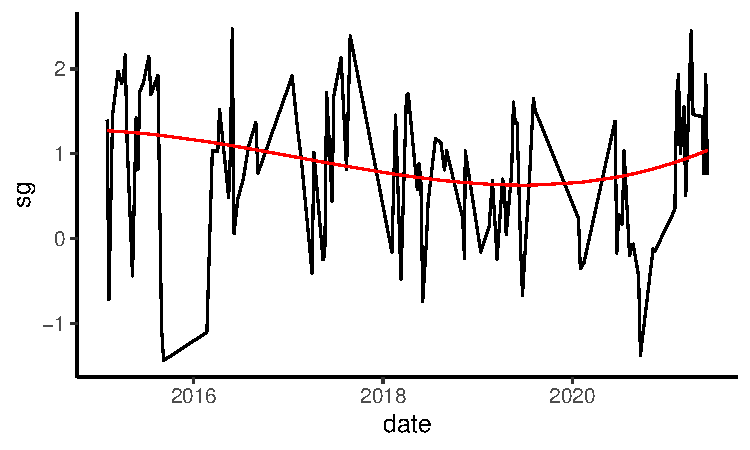
\includegraphics[width=\textwidth]{Figures/spieth_fitted_form.pdf}
    \caption{Fitted form of Jordan Spieth}
    \label{fig:fitted_form_spieth}
\end{minipage}%
\begin{minipage}{0.5\textwidth}
    \centering
    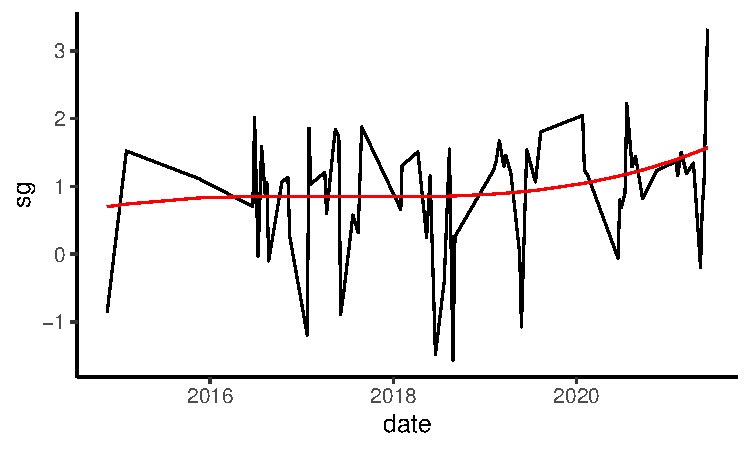
\includegraphics[width=\textwidth]{Figures/rahm_fitted_form.pdf}
    \caption{Fitted form of Jon Rahm}
    \label{fig:fitted_form_rahm}
\end{minipage}
\end{figure}

Figures \ref{fig:thomas_posterior_predictive}, \ref{fig:spieth_posterior_predictive}, \ref{fig:rahm_posterior_predictive} and \ref{fig:dechambeau_posterior_predictive} show a representation of the posterior predictive density versus empirical distribution of the residuals of the model for the players we looked at in Section 3.3 (model exploration). We notice that the model seems to fit very well to Thomas's data and well for Rahm, Spieth and DeChambeau. For a full posterior predictive check, one would have to use many samples and smoothing but this method gives an idea of the posterior predictive density.
\medskip\par
Figure \ref{fig:p_values} is a histogram the $p$-values of the players in the model. Only 1 player has a $p$-value outside $[0.025;0.975]$, which indicates that the model describes the data adequately well.

\begin{figure}[h]
\begin{minipage}{0.475\textwidth}
    \centering
    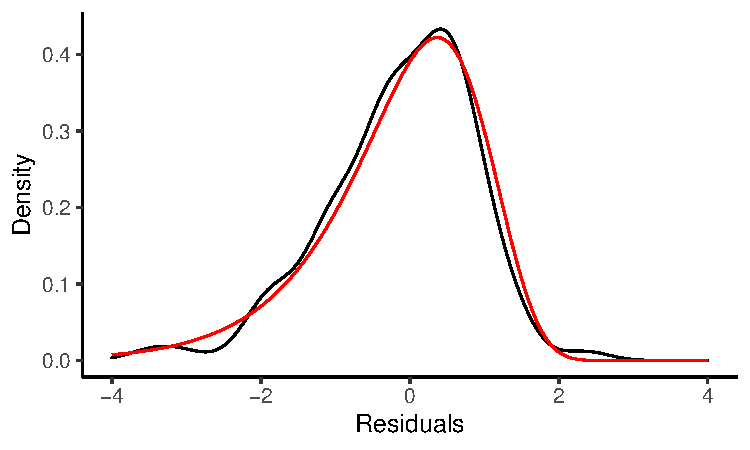
\includegraphics[width=1\textwidth]{Figures/posterior_predictive_thomas.pdf}
    \caption{A representative for the posterior predictive distribution for the residuals standardized strokes gained for for Justin Thomas}
    \label{fig:thomas_posterior_predictive}
\end{minipage}
\hspace{0.05\textwidth}
\begin{minipage}{0.475\textwidth}
    \centering
    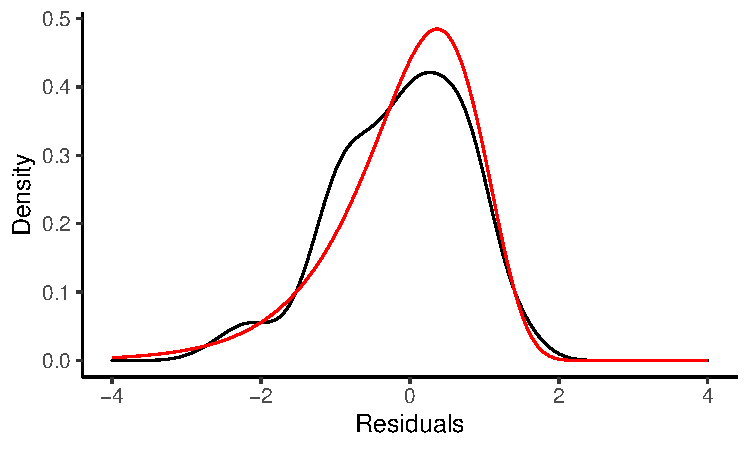
\includegraphics[width=1\textwidth]{Figures/posterior_predictive_spieth.pdf}
    \caption{A representative for the posterior predictive distribution for the residuals standardized strokes gained for for Jordan Spieth}
    \label{fig:spieth_posterior_predictive}
\end{minipage}
\end{figure}
%
\begin{figure}[h]
\begin{minipage}{0.475\textwidth}
    \centering
    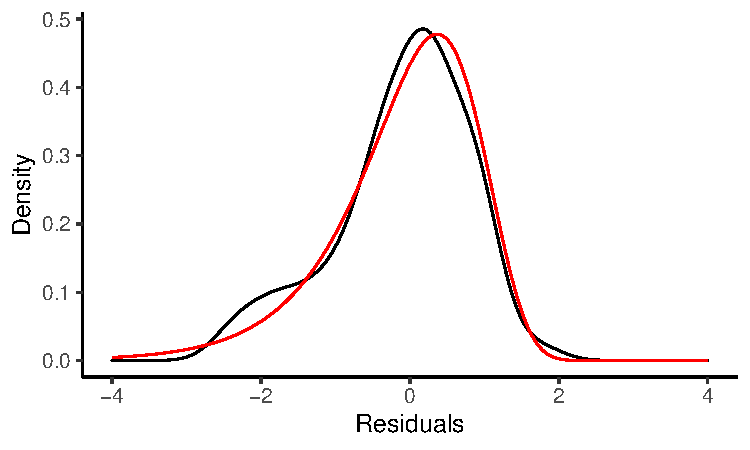
\includegraphics[width=1\textwidth]{Figures/posterior_predictive_rahm.pdf}
    \caption{A representative for the posterior predictive distribution for the residuals standardized strokes gained for for Jon Rahm}
    \label{fig:rahm_posterior_predictive}
\end{minipage}
\hspace{0.05\textwidth}
\begin{minipage}{0.475\textwidth}
    \centering
    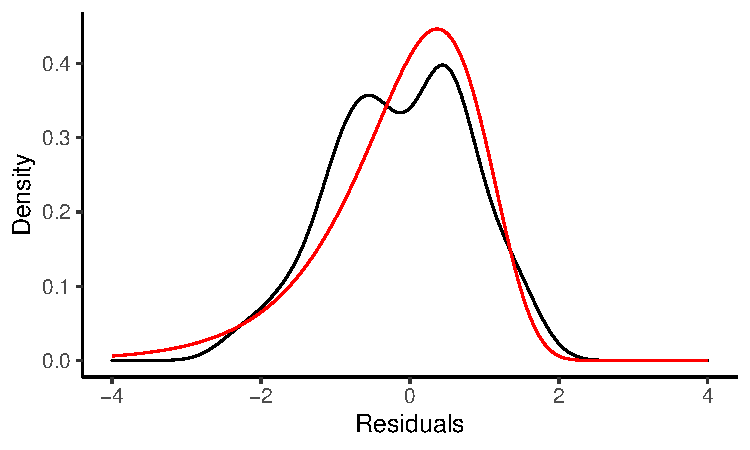
\includegraphics[width=1\textwidth]{Figures/posterior_predictive_dechambeau.pdf}
    \caption{A representative for the posterior predictive distribution for the residuals standardized strokes gained for Bryson DeChambeau}
    \label{fig:dechambeau_posterior_predictive}
\end{minipage}
\end{figure}
\begin{figure}
    \centering
    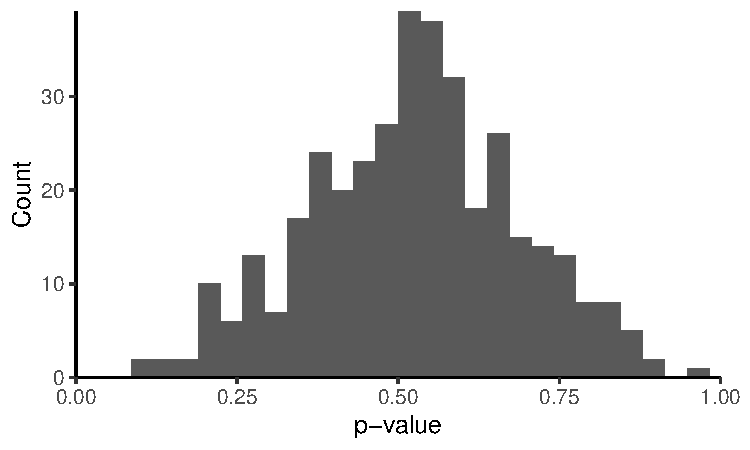
\includegraphics[width=4in]{Figures/p_values.pdf}
    \caption{A histogram of the Bayesian $p$-values for the players in the model.}
    \label{fig:p_values}
\end{figure}
\newpage
\null\newpage
\subsection{Posterior simulation - tournament results}
The 12 tournaments that were left out in the data were simulated according to the procedure described in section 2. Here we present the results for three of these tournaments for the full model along with a performance estimate of a random guessing model. These tournaments were chosen since the U.S. Open and The Open are two of the four so-called ''major'' tournaments every year and The Rocket Mortgage Classic was chosen to also showcase a smaller tournament. Table \ref{tab:predictions_full} shows the proportion of the correct guesses of the model for the tournaments for winners, top 10, top 25 and made cut. Table \ref{tab:predictions_random} shows the same for the random model. We note that the full model performs quite a lot better than the random model in all aspects.

\begin{table}[!h]
\centering
\caption{Performance of the full model on three tournaments that were left out in the fitting.}
\begin{tabular}[t]{lrrr}
\toprule
\textbf{Full model} & \textbf{U.S. Open} & \textbf{The Open} & \textbf{Rocket Classic}\\
\midrule
Correct winner & 100\% & 0\% & 0\% \\
Correct top 10 & 40\% & 50\% & 0\% \\
Correct top 25 & 36\% & 36\% & 40\% \\
Correct made cut & 51\% & 54\% & 57\% \\
\bottomrule
\end{tabular}
\label{tab:predictions_full}
\end{table}

\begin{table}[!h]
\centering
    \caption{Model performance for a random guess of player position.}
    \begin{tabular}[t]{lrrr}
    \toprule
    \textbf{Random guess} & \textbf{U.S. Open} & \textbf{The Open} & \textbf{Rocket Classic}\\
    \midrule
        Correct winner & 0.6\% & 1.3\% & 0.7\% \\
        Correct top 10 & 10.3\% & 10.7\% & 7.7\% \\
        Correct top 25 & 22.8\% & 22.8\% & 20.9\% \\
        Correct made cut & 50.5\% & 52.6\% & 49.7\% \\
    \bottomrule
    \end{tabular}
    \label{tab:predictions_random}
\end{table}

\newpage
\section{Discussions and conclusions}
Golf is a sport that is very hard to predict, as there are so many players competing at each tournament and because of the multiple factors that make a winner. The goal of this study was to be able to predict for winners and top players in tournaments on the PGA tour. To do that, we have come up with a measure of a player's quality in time and space, by using performance relative to the other players that are playing a given tournament. 
\medskip\par
By looking at the results, we have discovered that the model fits the data adequately well. The theoretical distributions seem to be reasonable. Of the three models that were compared, the most advanced model did the best in terms of DIC. It is very interesting to see that even though it has quite a lot more parameters than the other two models, it still performs better than the simpler models. It is convincing to look at the polynomial that is fit for the players we looked at in the study along with the Gumbel assumption on the residuals of the model. This task of modeling the performance of a golfer seems to be possible and we are able to capture some factors in a golfers performance with this method.
\medskip\par
Some ideas that seemed convincing at first did not work. One of these was a time series based model for the $SG$ variable. This model did not perform well, there was not enough correlation in $SG$ close in time to create a linear model. That model also assumed normality which was not found to be reasonable.
\medskip\par 
In practice, one would like to use the model at predicting for future tournaments on the PGA Tour, in online betting or such activities (although all gambling is discouraged) or just as a hobby. By looking at the simulations introduced, we saw that the model performs quite better than a random model, but would it help a sports better win bets?. It is good at predicting top 10, top 25 but it seems that it is harder to predict who make the cut.
\medskip\par
There are endless possibilities in trying to improve the model. It would be extremely interesting to incorporate a course fit to the player, f.ex. a player that hits it long performs well on a long course, a player that is good at playing in windy areas is good at courses by the sea etc. For this task to be completed, we would need more detailed data on a players strengths and weaknesses, however it would be possible.

\bibliographystyle{apalike} 
\bibliography{references} 

\newpage
\section{Appendix}
\subsection{Data manipulation}
\begin{knitrout}
\definecolor{shadecolor}{rgb}{0.969, 0.969, 0.969}\color{fgcolor}\begin{kframe}
\begin{alltt}
\hlcom{# manipulate_data.R}

\hlkwd{library}\hlstd{(readr)}
\hlkwd{library}\hlstd{(dplyr)}
\hlkwd{library}\hlstd{(here)}
\hlkwd{library}\hlstd{(tidyr)}
\hlkwd{library}\hlstd{(lubridate)}

\hlcom{# It is quite unnatural that the made cut rate is above 80%}
\hlstd{golf_dat} \hlkwb{<-} \hlkwd{read_csv}\hlstd{(}\hlkwd{here}\hlstd{(}\hlstr{"final_project"}\hlstd{,} \hlstr{"Data"} \hlstd{,} \hlstr{"pga_raw_data.csv"}\hlstd{))} \hlopt
    \hlkwd{group_by}\hlstd{(`tournament name`, date)} \hlopt \hlkwd{filter}\hlstd{(}\hlkwd{mean}\hlstd{(made_cut)} \hlopt{<=} \hlnum{0.8}\hlstd{)}

\hlstd{K} \hlkwb{<-} \hlnum{10}

\hlcom{# Make sure at least 10 data points per player }
\hlstd{sg_dat} \hlkwb{<-} \hlstd{golf_dat} \hlopt
    \hlkwd{group_by}\hlstd{(player)} \hlopt
    \hlkwd{filter}\hlstd{(}\hlkwd{n}\hlstd{()} \hlopt{>=} \hlnum{10}\hlstd{)} \hlopt
    \hlkwd{ungroup}\hlstd{()} \hlopt
    \hlkwd{rename}\hlstd{(}\hlkwc{tournament} \hlstd{=} \hlstr{"tournament name"}\hlstd{)} \hlopt
    \hlkwd{group_by}\hlstd{(tournament, date)} \hlopt
    \hlkwd{mutate}\hlstd{(}\hlkwc{average_strokes} \hlstd{= strokes}\hlopt{/}\hlstd{n_rounds,}
           \hlkwc{mean_strokes} \hlstd{=} \hlkwd{mean}\hlstd{(average_strokes),}
           \hlkwc{sg} \hlstd{= (}\hlkwd{mean}\hlstd{(average_strokes)}\hlopt{-}\hlstd{average_strokes)}\hlopt{/}\hlkwd{sd}\hlstd{(average_strokes))} \hlopt
    \hlkwd{filter}\hlstd{(}\hlopt{!}\hlkwd{is.na}\hlstd{(sg))} \hlopt
    \hlstd{ungroup} \hlopt
    \hlkwd{arrange}\hlstd{(date)}

\hlstd{cutoff_date} \hlkwb{<-} \hlstd{sg_dat} \hlopt \hlstd{ungroup} \hlopt
    \hlkwd{filter}\hlstd{(tournament} \hlopt{==} \hlstr{"U.S. Open"}\hlstd{,} \hlkwd{year}\hlstd{(date)} \hlopt{==} \hlnum{2021}\hlstd{)} \hlopt
    \hlkwd{slice}\hlstd{(}\hlnum{1}\hlstd{)} \hlopt \hlkwd{pull}\hlstd{(date)}

\hlstd{cutoff_players} \hlkwb{<-} \hlkwd{filter}\hlstd{(sg_dat, date} \hlopt{<} \hlstd{cutoff_date)} \hlopt \hlkwd{pull}\hlstd{(player)} \hlopt \hlstd{unique}

\hlstd{sg_dat} \hlkwb{<-} \hlstd{sg_dat} \hlopt \hlkwd{group_by}\hlstd{(player)} \hlopt
    \hlkwd{select}\hlstd{(player, tournament, date, pos, sg)} \hlopt
    \hlkwd{filter}\hlstd{(player} \hlopt \hlstd{cutoff_players)} \hlopt
    \hlkwd{mutate}\hlstd{(}\hlkwc{group} \hlstd{=} \hlkwd{group_indices}\hlstd{())} \hlopt
    \hlkwd{mutate}\hlstd{(}\hlkwc{t_star} \hlstd{=} \hlkwd{as.numeric}\hlstd{(date}\hlopt{-}\hlkwd{min}\hlstd{(date)),}
           \hlkwc{t} \hlstd{=} \hlnum{2}\hlopt{*}\hlstd{(t_star}\hlopt{-}\hlstd{(}\hlkwd{max}\hlstd{(t_star)}\hlopt{-}\hlkwd{min}\hlstd{(t_star))}\hlopt{/}\hlnum{2}\hlstd{)}\hlopt{/}
               \hlstd{(}\hlkwd{max}\hlstd{(t_star)}\hlopt{-}\hlkwd{min}\hlstd{(t_star)))} \hlopt
    \hlkwd{select}\hlstd{(}\hlkwd{c}\hlstd{(}\hlopt{-}\hlstd{t_star))} \hlopt
    \hlstd{ungroup}

\hlstd{sg_dat_cutoff} \hlkwb{<-} \hlstd{sg_dat} \hlopt \hlkwd{filter}\hlstd{(date} \hlopt{<} \hlstd{cutoff_date)}

\hlcom{# This is the data that the model is fitted to    }
\hlstd{sg_dat_cutoff} \hlopt \hlkwd{write_csv}\hlstd{(}\hlkwd{here}\hlstd{(}\hlstr{"final_project"}\hlstd{,} \hlstr{"Data"}\hlstd{,} \hlstr{"sg_dat_cutoff.csv"}\hlstd{))}
\hlcom{# This is the full dataset}
\hlstd{sg_dat} \hlopt \hlkwd{write_csv}\hlstd{(}\hlkwd{here}\hlstd{(}\hlstr{"final_project"}\hlstd{,} \hlstr{"Data"}\hlstd{,} \hlstr{"sg_dat.csv"}\hlstd{))}
\end{alltt}
\end{kframe}
\end{knitrout}

\subsection{Stan models}
\begin{knitrout}
\definecolor{shadecolor}{rgb}{0.969, 0.969, 0.969}\color{fgcolor}\begin{kframe}
\begin{alltt}
\hlcom{# baseline_model.stan}

data \{
  int<lower=0> N;
  vector[N] y;
\}

parameters \{
  real mu;
  real beta;
\}

model \{
  -y ~ \hlkwd{gumbel}(-mu, \hlkwd{exp}(beta));
\}
\end{alltt}
\end{kframe}
\end{knitrout}

\begin{knitrout}
\definecolor{shadecolor}{rgb}{0.969, 0.969, 0.969}\color{fgcolor}\begin{kframe}
\begin{alltt}
\hlcom{# intercept_only_model.stan}

data \{
  int<lower=0> N; // The number of data points
  int<lower=0> Q; // The number of players;
  
  //Data 
  vector[N] y;
  int<lower=1, upper=Q> g[N]; // Player playing given tournament
\}

transformed data \{
  vector[N] negative_y = -y;
\}

parameters \{
  vector[Q] mu;
  vector<lower=0>[Q] beta;
  
  real gamma_mu;
  real<lower=0> tau_mu;
  
  real gamma_beta;
  real<lower=0> tau_beta;
\}

model \{
  gamma_mu ~ \hlkwd{normal}(0, 5);
  tau_mu ~ \hlkwd{scaled_inv_chi_square}(5, 5);
  
  gamma_beta ~ \hlkwd{normal}(3,5);
  tau_beta ~ \hlkwd{scaled_inv_chi_square}(5,5);
  
  mu ~ \hlkwd{normal}(gamma_mu, tau_mu);
  beta ~ \hlkwd{normal}(gamma_beta, tau_beta);
  
  negative_y[1:N] ~ \hlkwd{gumbel}(-mu[g[1:N]], beta[g[1:N]]);
\}
\end{alltt}
\end{kframe}
\end{knitrout}

\begin{knitrout}
\definecolor{shadecolor}{rgb}{0.969, 0.969, 0.969}\color{fgcolor}\begin{kframe}
\begin{alltt}
\hlcom{# full_model.stan}

data \{
  int<lower=0> N; // The number of data points
  int<lower=0> Q; // The number of players;
  
  //Data 
  vector[N] y;
  
  // Covariates
  vector[N] t; // Time measured on [-1;1]
  int<lower=1, upper=Q> g[N]; // Player playing given tournament
\}

transformed data \{
  vector[N] negative_y = -y;
  
  vector[N] t_squared;
  vector[N] t_cubed;
  \hlkwd{for}(i in 1:N) \{
    t_squared[i] = t[i]*t[i];
    t_cubed[i] = t_squared[i]*t[i];
  \}
\}

parameters \{
  vector[Q] log_beta;
  
  matrix[Q, 4] alpha;
  
  vector[4] mu_alpha;
  vector<lower=0>[4] sigma2_alpha;

  real mu_beta;
  real<lower=0> sigma2_beta;
\}

model \{
  // Hyperpriors
  mu_beta ~ \hlkwd{normal}(1,5);
  sigma2_beta ~ \hlkwd{scaled_inv_chi_square}(1,5);
  
  mu_alpha ~ \hlkwd{normal}(0,5);
  sigma2_alpha ~ \hlkwd{scaled_inv_chi_square}(1,5);
  
  \hlkwd{for}(i in 1:Q) \{
    alpha[i,] ~ \hlkwd{normal}(mu_alpha, \hlkwd{sqrt}(sigma2_alpha));
  \}
  
  log_beta ~ \hlkwd{normal}(mu_beta, \hlkwd{sqrt}(sigma2_beta));
  
  \hlkwd{for}(n in 1:N) \{
    negative_y[n] ~ \hlkwd{gumbel}(-(alpha[g[n],1] + alpha[g[n],2]*t[n] +  
      alpha[g[n],3]*t_squared[n] +  alpha[g[n],4]*t_cubed[n]), 
        \hlkwd{exp}(log_beta[g[n]]));
  \}
\}
\end{alltt}
\end{kframe}
\end{knitrout}

\subsection{Running the models}
\begin{knitrout}
\definecolor{shadecolor}{rgb}{0.969, 0.969, 0.969}\color{fgcolor}\begin{kframe}
\begin{alltt}
\hlcom{# run_models.R}
\hlkwd{library}\hlstd{(cmdstanr)}
\hlkwd{library}\hlstd{(dplyr)}
\hlkwd{library}\hlstd{(here)}
\hlkwd{library}\hlstd{(readr)}

\hlstd{run_gumbel_model} \hlkwb{<-} \hlkwa{function}\hlstd{(}\hlkwc{model}\hlstd{,} \hlkwc{warmup} \hlstd{=} \hlnum{500}\hlstd{,} \hlkwc{iters} \hlstd{=} \hlnum{500}\hlstd{,} \hlkwc{chains} \hlstd{=} \hlnum{4}\hlstd{) \{}
    \hlkwd{set_cmdstan_path}\hlstd{(}\hlstr{"~/software/cmdstan"}\hlstd{)}
    \hlstd{sg_dat} \hlkwb{<-} \hlkwd{read_csv}\hlstd{(}\hlkwd{here}\hlstd{(}\hlstr{"final_project"}\hlstd{,} \hlstr{"Data"}\hlstd{,} \hlstr{"sg_dat_cutoff.csv"}\hlstd{))}

    \hlstd{Q} \hlkwb{<-} \hlkwd{length}\hlstd{(}\hlkwd{unique}\hlstd{(sg_dat}\hlopt{$}\hlstd{group))}

    \hlstd{stan_data} \hlkwb{<-} \hlkwd{list}\hlstd{(}
        \hlkwc{N} \hlstd{=} \hlkwd{nrow}\hlstd{(sg_dat),}
        \hlkwc{Q} \hlstd{= Q,}
        \hlkwc{y} \hlstd{= sg_dat}\hlopt{$}\hlstd{sg,}
        \hlkwc{g} \hlstd{= sg_dat}\hlopt{$}\hlstd{group,}
        \hlkwc{t}\hlstd{= sg_dat}\hlopt{$}\hlstd{t}
    \hlstd{)}

    \hlstd{mod} \hlkwb{<-} \hlkwd{cmdstan_model}\hlstd{(}\hlkwd{here}\hlstd{(}\hlstr{"final_project"}\hlstd{,} \hlstr{"Models"}\hlstd{,} \hlkwd{paste0}\hlstd{(model,}\hlstr{".stan"}\hlstd{)))}

    \hlstd{fit} \hlkwb{<-} \hlstd{mod}\hlopt{$}\hlkwd{sample}\hlstd{(}
        \hlkwc{data} \hlstd{= stan_data,}
        \hlkwc{show_messages} \hlstd{=} \hlnum{FALSE}\hlstd{,}
        \hlkwc{chains} \hlstd{= chains,}
        \hlkwc{parallel_chains} \hlstd{= chains,}
        \hlkwc{iter_sampling} \hlstd{= iters,}
        \hlkwc{iter_warmup} \hlstd{= warmup,}
        \hlkwc{max_treedepth} \hlstd{=} \hlnum{15}\hlstd{,}
        \hlkwc{init} \hlstd{=} \hlnum{0}\hlstd{,}
        \hlkwc{refresh} \hlstd{=} \hlnum{10}
    \hlstd{)}

    \hlstd{fit}\hlopt{$}\hlkwd{save_object}\hlstd{(}\hlkwc{file} \hlstd{=} \hlkwd{here}\hlstd{(}\hlstr{"final_project"}\hlstd{,} \hlstr{"Models"}\hlstd{,} \hlkwd{paste0}\hlstd{(model,} \hlstr{".rds"}\hlstd{)))}
\hlstd{\}}

\hlkwd{run_gumbel_model}\hlstd{(}\hlstr{"baseline_model"}\hlstd{)}
\hlkwd{run_gumbel_model}\hlstd{(}\hlstr{"intercept_only_model"}\hlstd{)}
\hlkwd{run_gumbel_model}\hlstd{(}\hlstr{"full_model"}\hlstd{)}
\end{alltt}
\end{kframe}
\end{knitrout}

\subsection{Data analysis}
\begin{knitrout}
\definecolor{shadecolor}{rgb}{0.969, 0.969, 0.969}\color{fgcolor}\begin{kframe}
\begin{alltt}
\hlcom{# simulate_tournament.R}

\hlstd{inv_gumbel} \hlkwb{<-} \hlkwa{function}\hlstd{(}\hlkwc{x}\hlstd{,} \hlkwc{mu}\hlstd{,}\hlkwc{beta}\hlstd{) \{}
    \hlstd{mu} \hlopt{+} \hlstd{beta}\hlopt{*}\hlkwd{log}\hlstd{(}\hlopt{-}\hlkwd{log}\hlstd{(x))}
\hlstd{\}}

\hlcom{# Full model}
\hlstd{simulate_tournament} \hlkwb{<-} \hlkwa{function}\hlstd{(}\hlkwc{tournament_name}\hlstd{,} \hlkwc{year}\hlstd{) \{}
    \hlstd{tournament_dat} \hlkwb{<-} \hlkwd{read_csv}\hlstd{(}\hlkwd{here}\hlstd{(}\hlstr{"final_project"}\hlstd{,} \hlstr{"Data"}\hlstd{,} \hlstr{"sg_dat.csv"}\hlstd{))} \hlopt
        \hlkwd{filter}\hlstd{(tournament} \hlopt{==} \hlstd{tournament_name,} \hlkwd{year}\hlstd{(date)} \hlopt{==} \hlstd{year)}

    \hlstd{mod} \hlkwb{<-} \hlkwd{read_rds}\hlstd{(}\hlkwd{here}\hlstd{(}\hlstr{"final_project"}\hlstd{,} \hlstr{"Models"}\hlstd{,} \hlstr{"gumbel_time_model.rds"}\hlstd{))}
    \hlstd{m} \hlkwb{<-} \hlstd{mod}\hlopt{$}\hlkwd{draws}\hlstd{()} \hlopt \hlstd{as_draws_df}
    \hlkwd{rm}\hlstd{(mod)}

    \hlstd{alpha_draws} \hlkwb{<-} \hlstd{m} \hlopt \hlkwd{spread_draws}\hlstd{(alpha[Q,i])} \hlopt
        \hlkwd{pivot_wider}\hlstd{(}\hlkwc{names_from} \hlstd{= i,}
                    \hlkwc{names_prefix} \hlstd{=} \hlstr{"alpha_"}\hlstd{,}
                    \hlkwc{values_from} \hlstd{= alpha)} \hlopt
        \hlstd{ungroup} \hlopt
        \hlkwd{rename}\hlstd{(}\hlkwc{group} \hlstd{= Q)} \hlopt
        \hlkwd{select}\hlstd{(group,} \hlkwd{matches}\hlstd{(}\hlstr{"alpha"}\hlstd{), .draw)}
    \hlstd{beta_draws} \hlkwb{<-} \hlstd{m} \hlopt \hlkwd{spread_draws}\hlstd{(log_beta[n])} \hlopt
        \hlkwd{mutate}\hlstd{(}\hlkwc{beta} \hlstd{=} \hlkwd{exp}\hlstd{(log_beta))} \hlopt
        \hlkwd{rename}\hlstd{(}\hlkwc{group} \hlstd{= n)} \hlopt
        \hlkwd{select}\hlstd{(group,beta, .draw)}

    \hlstd{parameter_draws} \hlkwb{<-} \hlkwd{left_join}\hlstd{(alpha_draws, beta_draws,} \hlkwc{by}\hlstd{=}\hlkwd{c}\hlstd{(}\hlstr{"group"}\hlstd{,} \hlstr{".draw"}\hlstd{))}

    \hlstd{cut} \hlkwb{<-} \hlkwd{length}\hlstd{(tournament_dat}\hlopt{$}\hlstd{pos[}\hlopt{!}\hlkwd{is.na}\hlstd{(tournament_dat}\hlopt{$}\hlstd{pos)])}

    \hlstd{tournament_dat} \hlopt
        \hlkwd{left_join}\hlstd{(parameter_draws,} \hlkwc{by}\hlstd{=}\hlstr{"group"}\hlstd{)} \hlopt
        \hlkwd{mutate}\hlstd{(}\hlkwc{rng} \hlstd{=} \hlkwd{runif}\hlstd{(}\hlkwd{n}\hlstd{()),}
               \hlkwc{mu} \hlstd{= alpha_1} \hlopt{+} \hlstd{t}\hlopt{*}\hlstd{alpha_2} \hlopt{+} \hlstd{t}\hlopt{^}\hlnum{2}\hlopt{*}\hlstd{alpha_3} \hlopt{+} \hlstd{t}\hlopt{^}\hlnum{3}\hlopt{*}\hlstd{alpha_4,}
               \hlkwc{predicted} \hlstd{=} \hlkwd{inv_gumbel}\hlstd{(rng, mu, beta),}
               \hlkwc{uniform_dist} \hlstd{= (sg}\hlopt{-}\hlkwd{inv_gumbel}\hlstd{(}\hlnum{0.025}\hlstd{,mu,beta))}\hlopt{/}
                   \hlstd{(}\hlkwd{inv_gumbel}\hlstd{(}\hlnum{0.975}\hlstd{, mu,beta)}\hlopt{-}\hlkwd{inv_gumbel}\hlstd{(}\hlnum{0.025}\hlstd{,mu,beta)))} \hlopt
        \hlkwd{group_by}\hlstd{(.draw)} \hlopt
        \hlkwd{arrange}\hlstd{(}\hlkwd{desc}\hlstd{(predicted))} \hlopt
        \hlkwd{mutate}\hlstd{(}\hlkwc{predicted_pos} \hlstd{=} \hlnum{1}\hlopt{:}\hlkwd{n}\hlstd{())} \hlopt
        \hlkwd{ungroup}\hlstd{()} \hlopt
        \hlkwd{group_by}\hlstd{(player)} \hlopt
        \hlkwd{summarise}\hlstd{(}\hlkwc{win_prob} \hlstd{=} \hlkwd{mean}\hlstd{(predicted_pos} \hlopt{==} \hlnum{1}\hlstd{),}
                  \hlkwc{top_10_prob} \hlstd{=} \hlkwd{mean}\hlstd{(predicted_pos} \hlopt{<=} \hlnum{10}\hlstd{),}
                  \hlkwc{top_25_prob} \hlstd{=} \hlkwd{mean}\hlstd{(predicted_pos} \hlopt{<=} \hlnum{25}\hlstd{),}
                  \hlkwc{made_cut_prob} \hlstd{=} \hlkwd{mean}\hlstd{(predicted_pos} \hlopt{<=} \hlstd{cut),}
                  \hlkwc{predicted_sg} \hlstd{=} \hlkwd{mean}\hlstd{(mu))} \hlopt
        \hlkwd{left_join}\hlstd{(tournament_dat,} \hlkwc{by}\hlstd{=}\hlstr{"player"}\hlstd{)} \hlopt
        \hlkwd{ungroup}\hlstd{()} \hlopt
        \hlkwd{arrange}\hlstd{(}\hlkwd{desc}\hlstd{(win_prob))} \hlopt
        \hlkwd{mutate}\hlstd{(}\hlkwc{predicted_pos} \hlstd{=} \hlkwd{c}\hlstd{(}\hlnum{1}\hlopt{:}\hlstd{cut,} \hlkwd{rep}\hlstd{(}\hlnum{NA}\hlstd{,} \hlkwd{n}\hlstd{()}\hlopt{-}\hlstd{cut)))} \hlopt
        \hlkwd{arrange}\hlstd{(predicted_pos)} \hlopt
        \hlkwd{select}\hlstd{(player, win_prob, top_10_prob, top_25_prob, made_cut_prob,}
               \hlstd{tournament, pos, predicted_pos, sg, predicted_sg)}
\hlstd{\}}

\hlcom{# Random model}
\hlstd{simulate_uniform} \hlkwb{<-} \hlkwa{function}\hlstd{(}\hlkwc{tournament_name}\hlstd{,} \hlkwc{year}\hlstd{) \{}
    \hlstd{tournament_dat} \hlkwb{<-} \hlkwd{read_csv}\hlstd{(}\hlkwd{here}\hlstd{(}\hlstr{"final_project"}\hlstd{,} \hlstr{"Data"}\hlstd{,} \hlstr{"sg_dat.csv"}\hlstd{))} \hlopt
        \hlkwd{filter}\hlstd{(tournament} \hlopt{==} \hlstd{tournament_name,} \hlkwd{year}\hlstd{(date)} \hlopt{==} \hlstd{year)}

    \hlstd{total_winners} \hlkwb{<-} \hlnum{0}
    \hlstd{total_top_10} \hlkwb{<-} \hlnum{0}
    \hlstd{total_top_25} \hlkwb{<-} \hlnum{0}
    \hlstd{total_made_cut} \hlkwb{<-} \hlnum{0}

    \hlstd{cut} \hlkwb{<-} \hlkwd{length}\hlstd{(tournament_dat}\hlopt{$}\hlstd{pos[}\hlopt{!}\hlkwd{is.na}\hlstd{(tournament_dat}\hlopt{$}\hlstd{pos)])}

    \hlstd{L} \hlkwb{<-} \hlnum{2000}
    \hlkwa{for}\hlstd{(i} \hlkwa{in} \hlnum{1}\hlopt{:}\hlstd{L) \{}
        \hlstd{simulation} \hlkwb{<-} \hlstd{tournament_dat} \hlopt \hlkwd{slice}\hlstd{(}\hlkwd{sample}\hlstd{(}\hlkwd{n}\hlstd{()))} \hlopt
            \hlkwd{mutate}\hlstd{(}\hlkwc{predicted_pos} \hlstd{=} \hlnum{1}\hlopt{:}\hlkwd{n}\hlstd{())}
        \hlstd{total_winners} \hlkwb{<-} \hlstd{total_winners} \hlopt{+} \hlkwd{nrow}\hlstd{(}\hlkwd{filter}\hlstd{(simulation, pos} \hlopt{==} \hlnum{1}\hlstd{,}
                                                     \hlstd{predicted_pos} \hlopt{==} \hlnum{1}\hlstd{))}
        \hlstd{total_top_10} \hlkwb{<-} \hlstd{total_top_10} \hlopt{+} \hlkwd{nrow}\hlstd{(}\hlkwd{filter}\hlstd{(simulation, pos} \hlopt{<=} \hlnum{10}\hlstd{,}
                                                   \hlstd{predicted_pos} \hlopt{<=} \hlnum{10}\hlstd{))}
        \hlstd{total_top_25} \hlkwb{<-} \hlstd{total_top_25} \hlopt{+} \hlkwd{nrow}\hlstd{(}\hlkwd{filter}\hlstd{(simulation, pos} \hlopt{<=} \hlnum{25}\hlstd{,}
                                                   \hlstd{predicted_pos} \hlopt{<=} \hlnum{25}\hlstd{))}
        \hlstd{total_made_cut} \hlkwb{<-} \hlstd{total_made_cut} \hlopt{+} \hlkwd{nrow}\hlstd{(}\hlkwd{filter}\hlstd{(simulation,}
                                                       \hlstd{pos} \hlopt{<=} \hlstd{cut,}
                                                       \hlstd{predicted_pos} \hlopt{<=} \hlstd{cut))}
    \hlstd{\}}

    \hlkwd{tibble}\hlstd{(}\hlkwc{prop_winners} \hlstd{= total_winners}\hlopt{/}\hlstd{L,}
         \hlkwc{prop_top_10} \hlstd{= total_top_10}\hlopt{/}\hlstd{(}\hlnum{10}\hlopt{*}\hlstd{L),}
         \hlkwc{prop_top_25} \hlstd{= total_top_25}\hlopt{/}\hlstd{(}\hlnum{25}\hlopt{*}\hlstd{L),}
         \hlkwc{prop_made_cut} \hlstd{= total_made_cut}\hlopt{/}\hlstd{(cut}\hlopt{*}\hlstd{L))}
\hlstd{\}}
\end{alltt}
\end{kframe}
\end{knitrout}

\begin{knitrout}
\definecolor{shadecolor}{rgb}{0.969, 0.969, 0.969}\color{fgcolor}\begin{kframe}
\begin{alltt}
\hlcom{# analyze_models.R}

\hlkwd{library}\hlstd{(posterior)}
\hlkwd{library}\hlstd{(tidyr)}
\hlkwd{library}\hlstd{(readr)}
\hlkwd{library}\hlstd{(dplyr)}
\hlkwd{library}\hlstd{(here)}
\hlkwd{library}\hlstd{(lubridate)}
\hlkwd{library}\hlstd{(rstan)}
\hlkwd{library}\hlstd{(tidybayes)}
\hlkwd{library}\hlstd{(latex2exp)}

\hlkwd{source}\hlstd{(}\hlkwd{here}\hlstd{(}\hlstr{"final_project"}\hlstd{,} \hlstr{"Scripts"}\hlstd{,} \hlstr{"simulate_tournament_gumbel.R"}\hlstd{))}
\hlkwd{theme_set}\hlstd{(}\hlkwd{theme_classic}\hlstd{(}\hlkwc{base_size} \hlstd{=} \hlnum{12}\hlstd{)} \hlopt{+} \hlkwd{theme}\hlstd{(}\hlkwc{legend.position} \hlstd{=} \hlstr{"bottom"}\hlstd{))}

\hlcom{# Reading in the model}
\hlstd{gumbel_time_model} \hlkwb{<-} \hlkwd{read_rds}\hlstd{(}\hlkwd{here}\hlstd{(}\hlstr{"final_project"}\hlstd{,} \hlstr{"Models"}\hlstd{,}
                                   \hlstr{"gumbel_time_model.rds"}\hlstd{))}
\hlstd{gumbel_time_m} \hlkwb{<-} \hlstd{gumbel_time_model}\hlopt{$}\hlkwd{draws}\hlstd{()} \hlopt \hlstd{as_draws_df}
\hlkwd{rm}\hlstd{(gumbel_time_model)}

\hlcom{# Calculating parameter estimates}
\hlstd{posterior_alpha_estimates} \hlkwb{<-} \hlstd{gumbel_time_m} \hlopt \hlkwd{spread_draws}\hlstd{(alpha[Q,i])} \hlopt
    \hlkwd{group_by}\hlstd{(Q,i)} \hlopt
    \hlkwd{summarise}\hlstd{(}\hlkwc{lower_95} \hlstd{=} \hlkwd{quantile}\hlstd{(alpha,} \hlnum{0.025}\hlstd{),}
              \hlkwc{median} \hlstd{=} \hlkwd{quantile}\hlstd{(alpha,}\hlnum{0.5}\hlstd{),}
              \hlkwc{upper_95} \hlstd{=} \hlkwd{quantile}\hlstd{(alpha,}\hlnum{0.975}\hlstd{))} \hlopt
    \hlkwd{select}\hlstd{(Q,i,median)} \hlopt
    \hlkwd{pivot_wider}\hlstd{(}\hlkwc{names_from} \hlstd{= i,}
                \hlkwc{names_prefix} \hlstd{=} \hlstr{"alpha_"}\hlstd{,}
                \hlkwc{values_from} \hlstd{= median)} \hlopt
    \hlkwd{rename}\hlstd{(}\hlkwc{group} \hlstd{= Q)} \hlopt
    \hlstd{ungroup}

\hlstd{posterior_beta_estimates} \hlkwb{<-} \hlstd{gumbel_time_m} \hlopt \hlkwd{spread_draws}\hlstd{(log_beta[group])} \hlopt
    \hlkwd{mutate}\hlstd{(}\hlkwc{beta} \hlstd{=} \hlkwd{exp}\hlstd{(log_beta))} \hlopt
    \hlkwd{group_by}\hlstd{(group)} \hlopt
    \hlkwd{summarise}\hlstd{(}\hlkwc{beta} \hlstd{=} \hlkwd{quantile}\hlstd{(beta,} \hlnum{0.5}\hlstd{))}\hlopt
    \hlstd{ungroup}

\hlstd{hyperparameter_estimates} \hlkwb{<-} \hlstd{gumbel_time_m} \hlopt \hlkwd{select}\hlstd{(}\hlkwd{matches}\hlstd{(}\hlstr{"mu_alpha"}\hlstd{),}
                                                     \hlkwd{matches}\hlstd{(}\hlstr{"sigma2_alpha"}\hlstd{),}
                                                     \hlstd{mu_beta, sigma2_beta)} \hlopt
    \hlkwd{rename}\hlstd{(}\hlkwc{sigma_alpha_1} \hlstd{=} \hlstr{"sigma2_alpha[1]"}\hlstd{,}
           \hlkwc{sigma_alpha_2} \hlstd{=} \hlstr{"sigma2_alpha[2]"}\hlstd{,}
           \hlkwc{sigma_alpha_3} \hlstd{=} \hlstr{"sigma2_alpha[3]"}\hlstd{,}
           \hlkwc{sigma_alpha_4} \hlstd{=} \hlstr{"sigma2_alpha[4]"}\hlstd{,}
           \hlkwc{mu_alpha_1} \hlstd{=} \hlstr{"mu_alpha[1]"}\hlstd{,}
           \hlkwc{mu_alpha_2} \hlstd{=} \hlstr{"mu_alpha[2]"}\hlstd{,}
           \hlkwc{mu_alpha_3} \hlstd{=} \hlstr{"mu_alpha[3]"}\hlstd{,}
           \hlkwc{mu_alpha_4} \hlstd{=} \hlstr{"mu_alpha[4]"}\hlstd{,}
           \hlkwc{sigma_beta} \hlstd{= sigma2_beta)} \hlopt
    \hlkwd{as_tibble}\hlstd{()} \hlopt
    \hlkwd{mutate}\hlstd{(}\hlkwc{sigma_alpha_1} \hlstd{=} \hlkwd{sqrt}\hlstd{(sigma_alpha_1),}
           \hlkwc{sigma_alpha_2} \hlstd{=} \hlkwd{sqrt}\hlstd{(sigma_alpha_2),}
           \hlkwc{sigma_alpha_3} \hlstd{=} \hlkwd{sqrt}\hlstd{(sigma_alpha_3),}
           \hlkwc{sigma_alpha_4} \hlstd{=} \hlkwd{sqrt}\hlstd{(sigma_alpha_4),}
           \hlkwc{sigma_beta} \hlstd{=} \hlkwd{sqrt}\hlstd{(sigma_beta))} \hlopt
    \hlkwd{mutate}\hlstd{(}\hlkwc{draw} \hlstd{=} \hlnum{1}\hlopt{:}\hlkwd{n}\hlstd{())} \hlopt
    \hlkwd{pivot_longer}\hlstd{(}\hlkwd{c}\hlstd{(}\hlopt{-}\hlstd{draw),} \hlkwc{names_to}\hlstd{=}\hlstr{"parameter"}\hlstd{)} \hlopt
    \hlkwd{group_by}\hlstd{(parameter)} \hlopt
    \hlkwd{summarise}\hlstd{(}\hlkwc{lower_95} \hlstd{=} \hlkwd{quantile}\hlstd{(value,} \hlnum{0.025}\hlstd{),}
              \hlkwc{median} \hlstd{=} \hlkwd{quantile}\hlstd{(value,}\hlnum{0.5}\hlstd{),}
              \hlkwc{upper_95} \hlstd{=} \hlkwd{quantile}\hlstd{(value,}\hlnum{0.975}\hlstd{))} \hlopt
    \hlkwd{slice}\hlstd{(}\hlkwd{c}\hlstd{(}\hlnum{1}\hlstd{,}\hlnum{6}\hlstd{,}\hlnum{2}\hlstd{,}\hlnum{7}\hlstd{,}\hlnum{3}\hlstd{,}\hlnum{8}\hlstd{,}\hlnum{4}\hlstd{,}\hlnum{9}\hlstd{,}\hlnum{5}\hlstd{,}\hlnum{10}\hlstd{))} \hlopt
    \hlkwd{mutate}\hlstd{(}\hlkwc{parameter} \hlstd{=} \hlkwd{paste0}\hlstd{(}\hlstr{"$\textbackslash{}\textbackslash{}"}\hlstd{,parameter,} \hlstr{"\}$"}\hlstd{),}
           \hlkwc{parameter} \hlstd{=} \hlkwd{gsub}\hlstd{(}\hlstr{"alpha"}\hlstd{,} \hlstr{"\{\textbackslash{}\textbackslash{}\textbackslash{}\textbackslash{}alpha"}\hlstd{, parameter),}
           \hlkwc{parameter} \hlstd{=} \hlkwd{gsub}\hlstd{(}\hlstr{"beta"}\hlstd{,} \hlstr{"\{\textbackslash{}\textbackslash{}\textbackslash{}\textbackslash{}beta"}\hlstd{, parameter))} \hlopt
    \hlkwd{rename}\hlstd{(}\hlkwc{Parameter} \hlstd{= parameter,}
           \hlstr{"Lower 95\textbackslash{}\textbackslash{}%"} \hlstd{= lower_95,}
           \hlstr{"Posterior median"} \hlstd{= median,}
           \hlstr{"Upper 95\textbackslash{}\textbackslash{}%"} \hlstd{= upper_95)}

\hlkwd{kable}\hlstd{(hyperparameter_estimates)}

\hlstd{alpha_draws} \hlkwb{<-} \hlstd{gumbel_time_m} \hlopt \hlkwd{spread_draws}\hlstd{(alpha[group,i])} \hlopt
    \hlkwd{pivot_wider}\hlstd{(}\hlkwc{names_from} \hlstd{= i,}
                \hlkwc{names_prefix} \hlstd{=} \hlstr{"alpha_"}\hlstd{,}
                \hlkwc{values_from} \hlstd{= alpha)} \hlopt
    \hlstd{ungroup} \hlopt
    \hlkwd{select}\hlstd{(}\hlkwd{c}\hlstd{(}\hlopt{-}\hlstd{.chain,} \hlopt{-}\hlstd{.iteration))}
\hlstd{beta_draws} \hlkwb{<-} \hlstd{gumbel_time_m} \hlopt \hlkwd{spread_draws}\hlstd{(log_beta[group])} \hlopt
    \hlkwd{mutate}\hlstd{(}\hlkwc{beta} \hlstd{=} \hlkwd{exp}\hlstd{(log_beta))} \hlopt
    \hlkwd{select}\hlstd{(}\hlkwd{c}\hlstd{(}\hlopt{-}\hlstd{.chain,}\hlopt{-}\hlstd{.iteration,}\hlopt{-}\hlstd{log_beta))}

\hlstd{parameter_draws} \hlkwb{<-} \hlkwd{left_join}\hlstd{(alpha_draws, beta_draws,} \hlkwc{by}\hlstd{=}\hlkwd{c}\hlstd{(}\hlstr{"group"}\hlstd{,}\hlstr{".draw"}\hlstd{))}

\hlstd{sg_dat} \hlkwb{<-} \hlkwd{read_csv}\hlstd{(}\hlkwd{here}\hlstd{(}\hlstr{"final_project"}\hlstd{,} \hlstr{"Data"}\hlstd{,} \hlstr{"sg_dat.csv"}\hlstd{))}
\hlstd{sg_dat_cutoff} \hlkwb{<-} \hlkwd{read_csv}\hlstd{(}\hlkwd{here}\hlstd{(}\hlstr{"final_project"}\hlstd{,} \hlstr{"Data"}\hlstd{,} \hlstr{"sg_dat_cutoff.csv"}\hlstd{))}

\hlstd{mirror_gumbel_pdf} \hlkwb{<-} \hlkwa{function}\hlstd{(}\hlkwc{y}\hlstd{,} \hlkwc{mu}\hlstd{,}\hlkwc{beta}\hlstd{) \{}
    \hlstd{z} \hlkwb{=} \hlstd{(mu}\hlopt{-}\hlstd{y)}\hlopt{/}\hlstd{beta}
    \hlnum{1}\hlopt{/}\hlstd{beta}\hlopt{*}\hlkwd{exp}\hlstd{(}\hlopt{-}\hlstd{z}\hlopt{-}\hlkwd{exp}\hlstd{(}\hlopt{-}\hlstd{z))}
\hlstd{\}}

\hlstd{mirror_gumbel_cdf} \hlkwb{<-} \hlkwa{function}\hlstd{(}\hlkwc{y}\hlstd{,} \hlkwc{mu}\hlstd{,} \hlkwc{beta}\hlstd{) \{}
    \hlstd{z} \hlkwb{=} \hlstd{(mu}\hlopt{-}\hlstd{y)}\hlopt{/}\hlstd{beta}
    \hlkwd{exp}\hlstd{(}\hlopt{-}\hlkwd{exp}\hlstd{(}\hlopt{-}\hlstd{z))}
\hlstd{\}}

\hlstd{inverse_mirror_gumbel} \hlkwb{<-} \hlkwa{function}\hlstd{(}\hlkwc{p}\hlstd{,} \hlkwc{mu}\hlstd{,} \hlkwc{beta}\hlstd{) \{}
    \hlstd{beta}\hlopt{*}\hlkwd{log}\hlstd{(}\hlopt{-}\hlkwd{log}\hlstd{(p))}\hlopt{+}\hlstd{mu}
\hlstd{\}}

\hlcom{# Note that predicted is calculated according to scaling by }
\hlcom{# adding beta*log(log(2))}
\hlstd{player_predictions} \hlkwb{<-} \hlstd{sg_dat_cutoff} \hlopt
    \hlkwd{left_join}\hlstd{(posterior_alpha_estimates,} \hlkwc{by}\hlstd{=}\hlkwd{c}\hlstd{(}\hlstr{"group"}\hlstd{))} \hlopt
    \hlkwd{left_join}\hlstd{(posterior_beta_estimates,} \hlkwc{by}\hlstd{=}\hlkwd{c}\hlstd{(}\hlstr{"group"}\hlstd{))} \hlopt
    \hlkwd{mutate}\hlstd{(}\hlkwc{mu} \hlstd{= alpha_1} \hlopt{+} \hlstd{alpha_2}\hlopt{*}\hlstd{t} \hlopt{+} \hlstd{alpha_3}\hlopt{*}\hlstd{t}\hlopt{^}\hlnum{2} \hlopt{+} \hlstd{alpha_4}\hlopt{*}\hlstd{t}\hlopt{^}\hlnum{3}\hlstd{,}
           \hlkwc{predicted} \hlstd{= mu}\hlopt{+}\hlstd{beta}\hlopt{*}\hlkwd{log}\hlstd{(}\hlkwd{log}\hlstd{(}\hlnum{2}\hlstd{)),}
           \hlkwc{quantile} \hlstd{=} \hlkwd{mirror_gumbel_cdf}\hlstd{(sg, mu, beta),}
           \hlkwc{residuals} \hlstd{= sg}\hlopt{-}\hlstd{predicted)}

\hlstd{dens} \hlkwb{<-} \hlkwa{function}\hlstd{(}\hlkwc{fitted_player}\hlstd{,} \hlkwc{show_fit} \hlstd{= T) \{}
    \hlstd{index} \hlkwb{<-} \hlstd{sg_dat} \hlopt \hlkwd{filter}\hlstd{(player} \hlopt{==} \hlstd{fitted_player)} \hlopt \hlkwd{pull}\hlstd{(group)} \hlopt
        \hlkwd{unique}\hlstd{()}
    \hlstd{player_density} \hlkwb{<-} \hlkwd{tibble}\hlstd{(}\hlkwc{t}\hlstd{=}\hlkwd{seq}\hlstd{(}\hlopt{-}\hlnum{4}\hlstd{,}\hlnum{4}\hlstd{,}\hlnum{0.01}\hlstd{),}
                             \hlkwc{density}\hlstd{=}\hlkwd{mirror_gumbel_pdf}\hlstd{(t,}
                                       \hlopt{-}\hlkwd{log}\hlstd{(}\hlkwd{log}\hlstd{(}\hlnum{2}\hlstd{)),}
                                       \hlstd{posterior_beta_estimates}\hlopt{$}\hlstd{beta[index]))}
    \hlstd{p} \hlkwb{<-} \hlstd{player_predictions} \hlopt \hlkwd{filter}\hlstd{(player} \hlopt{==} \hlstd{fitted_player)} \hlopt
        \hlkwd{ggplot}\hlstd{()} \hlopt{+} \hlkwd{coord_cartesian}\hlstd{(}\hlkwc{xlim}\hlstd{=}\hlkwd{c}\hlstd{(}\hlopt{-}\hlnum{4}\hlstd{,}\hlnum{4}\hlstd{))} \hlopt{+}
        \hlkwd{geom_density}\hlstd{(}\hlkwd{aes}\hlstd{(}\hlkwc{x}\hlstd{=residuals))} \hlopt{+}
        \hlkwd{xlab}\hlstd{(}\hlstr{"Residuals"}\hlstd{)} \hlopt{+}
        \hlkwd{ylab}\hlstd{(}\hlstr{"Density"}\hlstd{)}

    \hlkwa{if}\hlstd{(show_fit) p} \hlkwb{<-} \hlstd{p}\hlopt{+}\hlkwd{geom_line}\hlstd{(}\hlkwc{data}\hlstd{=player_density,} \hlkwd{aes}\hlstd{(}\hlkwc{x}\hlstd{=t,}\hlkwc{y}\hlstd{=density),} \hlkwc{color}\hlstd{=}\hlstr{"red"}\hlstd{)}
    \hlstd{p}
\hlstd{\}}

\hlkwd{dens}\hlstd{(}\hlstr{"Justin Thomas"}\hlstd{)}
\hlkwd{ggsave}\hlstd{(}\hlkwd{here}\hlstd{(}\hlstr{"final_project"}\hlstd{,} \hlstr{"Report"}\hlstd{,} \hlstr{"Figures"}\hlstd{,}
            \hlstr{"posterior_predictive_thomas.pdf"}\hlstd{),} \hlkwc{width}\hlstd{=}\hlnum{5}\hlstd{,}\hlkwc{height}\hlstd{=}\hlnum{3}\hlstd{,} \hlkwc{device}\hlstd{=}\hlstr{"pdf"}\hlstd{)}
\hlkwd{dens}\hlstd{(}\hlstr{"Jon Rahm"}\hlstd{)}
\hlkwd{ggsave}\hlstd{(}\hlkwd{here}\hlstd{(}\hlstr{"final_project"}\hlstd{,} \hlstr{"Report"}\hlstd{,} \hlstr{"Figures"}\hlstd{,}
            \hlstr{"posterior_predictive_rahm.pdf"}\hlstd{),} \hlkwc{width}\hlstd{=}\hlnum{5}\hlstd{,}\hlkwc{height}\hlstd{=}\hlnum{3}\hlstd{,} \hlkwc{device}\hlstd{=}\hlstr{"pdf"}\hlstd{)}

\hlkwd{dens}\hlstd{(}\hlstr{"Jon Rahm"}\hlstd{,} \hlkwc{show_fit} \hlstd{= F)}
\hlkwd{ggsave}\hlstd{(}\hlkwd{here}\hlstd{(}\hlstr{"final_project"}\hlstd{,} \hlstr{"Report"}\hlstd{,} \hlstr{"Figures"}\hlstd{,}
            \hlstr{"rahm_empirical_density.pdf"}\hlstd{),} \hlkwc{width}\hlstd{=}\hlnum{5}\hlstd{,} \hlkwc{height}\hlstd{=}\hlnum{3}\hlstd{,} \hlkwc{device}\hlstd{=}\hlstr{"pdf"}\hlstd{)}

\hlkwd{dens}\hlstd{(}\hlstr{"Jordan Spieth"}\hlstd{,} \hlkwc{show_fit} \hlstd{= F)}
\hlkwd{ggsave}\hlstd{(}\hlkwd{here}\hlstd{(}\hlstr{"final_project"}\hlstd{,} \hlstr{"Report"}\hlstd{,} \hlstr{"Figures"}\hlstd{,}
            \hlstr{"empirical_density_spieth.pdf"}\hlstd{),} \hlkwc{width}\hlstd{=}\hlnum{5}\hlstd{,} \hlkwc{height}\hlstd{=}\hlnum{3}\hlstd{,} \hlkwc{device}\hlstd{=}\hlstr{"pdf"}\hlstd{)}

\hlkwd{dens}\hlstd{(}\hlstr{"Dustin Johnson"}\hlstd{)}
\hlkwd{dens}\hlstd{(}\hlstr{"Jordan Spieth"}\hlstd{)}
\hlkwd{ggsave}\hlstd{(}\hlkwd{here}\hlstd{(}\hlstr{"final_project"}\hlstd{,} \hlstr{"Report"}\hlstd{,} \hlstr{"Figures"}\hlstd{,}
            \hlstr{"posterior_predictive_spieth.pdf"}\hlstd{),} \hlkwc{width}\hlstd{=}\hlnum{5}\hlstd{,} \hlkwc{height}\hlstd{=}\hlnum{3}\hlstd{,} \hlkwc{device}\hlstd{=}\hlstr{"pdf"}\hlstd{)}

\hlkwd{dens}\hlstd{(}\hlstr{"Bryson DeChambeau"}\hlstd{)}
\hlkwd{ggsave}\hlstd{(}\hlkwd{here}\hlstd{(}\hlstr{"final_project"}\hlstd{,} \hlstr{"Report"}\hlstd{,} \hlstr{"Figures"}\hlstd{,}
            \hlstr{"posterior_predictive_dechambeau.pdf"}\hlstd{),} \hlkwc{width}\hlstd{=}\hlnum{5}\hlstd{,}\hlkwc{height}\hlstd{=}\hlnum{3}\hlstd{,} \hlkwc{device}\hlstd{=}\hlstr{"pdf"}\hlstd{)}
\hlkwd{dens}\hlstd{(}\hlstr{"Sandy Lyle"}\hlstd{)}

\hlstd{player_predictions} \hlopt \hlkwd{filter}\hlstd{(player} \hlopt{==} \hlstr{"Justin Thomas"}\hlstd{)} \hlopt
    \hlkwd{ggplot}\hlstd{(}\hlkwd{aes}\hlstd{(}\hlkwc{x}\hlstd{=residuals))} \hlopt{+} \hlkwd{geom_density}\hlstd{()} \hlopt{+}
    \hlkwd{geom_line}\hlstd{()}

\hlstd{p} \hlkwb{<-} \hlstd{player_predictions} \hlopt \hlkwd{filter}\hlstd{(player} \hlopt{==} \hlstr{"Jordan Spieth"}\hlstd{)} \hlopt
    \hlkwd{ggplot}\hlstd{()} \hlopt{+} \hlkwd{geom_line}\hlstd{(}\hlkwd{aes}\hlstd{(}\hlkwc{x}\hlstd{=date,}\hlkwc{y}\hlstd{=sg))} \hlopt{+}
    \hlkwd{geom_line}\hlstd{(}\hlkwd{aes}\hlstd{(}\hlkwc{x}\hlstd{=date,}\hlkwc{y}\hlstd{=predicted),} \hlkwc{color}\hlstd{=}\hlstr{'red'}\hlstd{)}
\hlkwd{ggsave}\hlstd{(}\hlkwd{here}\hlstd{(}\hlstr{"final_project"}\hlstd{,} \hlstr{"Report"}\hlstd{,} \hlstr{"Figures"}\hlstd{,} \hlstr{"spieth_fitted_form.pdf"}\hlstd{),}
       \hlstd{p,} \hlkwc{width}\hlstd{=}\hlnum{5}\hlstd{,} \hlkwc{height}\hlstd{=}\hlnum{3}\hlstd{,} \hlkwc{device}\hlstd{=}\hlstr{"pdf"}\hlstd{)}

\hlstd{p} \hlkwb{<-} \hlstd{player_predictions} \hlopt \hlkwd{filter}\hlstd{(player} \hlopt{==} \hlstr{"Bryson DeChambeau"}\hlstd{)} \hlopt
    \hlkwd{ggplot}\hlstd{()} \hlopt{+} \hlkwd{geom_line}\hlstd{(}\hlkwd{aes}\hlstd{(}\hlkwc{x}\hlstd{=date,}\hlkwc{y}\hlstd{=sg))}\hlcom{# + }
    \hlcom{#geom_line(aes(x=date,y=predicted), color='red')}
\hlkwd{ggsave}\hlstd{(}\hlkwd{here}\hlstd{(}\hlstr{"final_project"}\hlstd{,} \hlstr{"Report"}\hlstd{,} \hlstr{"Figures"}\hlstd{,} \hlstr{"dechambeau_sg.pdf"}\hlstd{),}
       \hlstd{p,} \hlkwc{width}\hlstd{=}\hlnum{5}\hlstd{,} \hlkwc{height}\hlstd{=}\hlnum{3}\hlstd{,} \hlkwc{device}\hlstd{=}\hlstr{"pdf"}\hlstd{)}

\hlkwd{ggsave}\hlstd{(}\hlkwd{here}\hlstd{(}\hlstr{"final_project"}\hlstd{,} \hlstr{"Report"}\hlstd{,} \hlstr{"Figures"}\hlstd{,} \hlstr{"dechambeau_fitted_form.pdf"}\hlstd{),}
       \hlstd{p,} \hlkwc{width}\hlstd{=}\hlnum{5}\hlstd{,} \hlkwc{height}\hlstd{=}\hlnum{3}\hlstd{,} \hlkwc{device}\hlstd{=}\hlstr{"pdf"}\hlstd{)}

\hlstd{p} \hlkwb{<-} \hlstd{player_predictions} \hlopt \hlkwd{filter}\hlstd{(player} \hlopt{==} \hlstr{"Jon Rahm"}\hlstd{)} \hlopt
    \hlkwd{ggplot}\hlstd{()} \hlopt{+} \hlkwd{geom_line}\hlstd{(}\hlkwd{aes}\hlstd{(}\hlkwc{x}\hlstd{=date,}\hlkwc{y}\hlstd{=sg))}
\hlkwd{ggsave}\hlstd{(}\hlkwd{here}\hlstd{(}\hlstr{"final_project"}\hlstd{,} \hlstr{"Report"}\hlstd{,} \hlstr{"Figures"}\hlstd{,} \hlstr{"rahm_sg.pdf"}\hlstd{),}
       \hlstd{p,} \hlkwc{width}\hlstd{=}\hlnum{5}\hlstd{,} \hlkwc{height}\hlstd{=}\hlnum{3}\hlstd{,} \hlkwc{device}\hlstd{=}\hlstr{"pdf"}\hlstd{)}

\hlkwd{ggsave}\hlstd{(}\hlkwd{here}\hlstd{(}\hlstr{"final_project"}\hlstd{,} \hlstr{"Report"}\hlstd{,} \hlstr{"Figures"}\hlstd{,} \hlstr{"rahm_fitted_form.pdf"}\hlstd{),}
       \hlstd{p,} \hlkwc{width}\hlstd{=}\hlnum{5}\hlstd{,} \hlkwc{height}\hlstd{=}\hlnum{3}\hlstd{,} \hlkwc{device}\hlstd{=}\hlstr{"pdf"}\hlstd{)}

\hlstd{mirror_gumbel_pdf} \hlkwb{<-} \hlkwa{function}\hlstd{(}\hlkwc{y}\hlstd{,} \hlkwc{mu}\hlstd{,}\hlkwc{beta}\hlstd{) \{}
    \hlstd{z} \hlkwb{=} \hlstd{(mu}\hlopt{-}\hlstd{y)}\hlopt{/}\hlstd{beta}
    \hlnum{1}\hlopt{/}\hlstd{beta}\hlopt{*}\hlkwd{exp}\hlstd{(}\hlopt{-}\hlstd{z}\hlopt{-}\hlkwd{exp}\hlstd{(}\hlopt{-}\hlstd{z))}
\hlstd{\}}

\hlstd{mirror_gumbel_cdf} \hlkwb{<-} \hlkwa{function}\hlstd{(}\hlkwc{y}\hlstd{,} \hlkwc{mu}\hlstd{,} \hlkwc{beta}\hlstd{) \{}
    \hlstd{z} \hlkwb{=} \hlstd{(mu}\hlopt{-}\hlstd{y)}\hlopt{/}\hlstd{beta}
    \hlkwd{exp}\hlstd{(}\hlopt{-}\hlkwd{exp}\hlstd{(}\hlopt{-}\hlstd{z))}
\hlstd{\}}

\hlcom{# Calculating the DIC etc.}
\hlstd{model_summary} \hlkwb{<-} \hlkwa{function}\hlstd{(}\hlkwc{m}\hlstd{,} \hlkwc{dat}\hlstd{) \{}
    \hlstd{posterior_alpha_estimates} \hlkwb{<-} \hlstd{m} \hlopt \hlkwd{spread_draws}\hlstd{(alpha[Q,i])} \hlopt
        \hlkwd{group_by}\hlstd{(Q,i)} \hlopt
        \hlkwd{summarise}\hlstd{(}\hlkwc{lower_95} \hlstd{=} \hlkwd{quantile}\hlstd{(alpha,} \hlnum{0.025}\hlstd{),}
                  \hlkwc{median} \hlstd{=} \hlkwd{quantile}\hlstd{(alpha,}\hlnum{0.5}\hlstd{),}
                  \hlkwc{upper_95} \hlstd{=} \hlkwd{quantile}\hlstd{(alpha,}\hlnum{0.975}\hlstd{))} \hlopt
        \hlkwd{select}\hlstd{(Q,i,median)} \hlopt
        \hlkwd{pivot_wider}\hlstd{(}\hlkwc{names_from} \hlstd{= i,}
                    \hlkwc{names_prefix} \hlstd{=} \hlstr{"alpha_"}\hlstd{,}
                    \hlkwc{values_from} \hlstd{= median)} \hlopt
        \hlkwd{rename}\hlstd{(}\hlkwc{group} \hlstd{= Q)} \hlopt
        \hlstd{ungroup}

    \hlstd{posterior_beta_estimates} \hlkwb{<-} \hlstd{m} \hlopt \hlkwd{spread_draws}\hlstd{(beta[n])} \hlopt
        \hlkwd{group_by}\hlstd{(n)} \hlopt
        \hlkwd{summarise}\hlstd{(}\hlkwc{beta} \hlstd{=} \hlkwd{quantile}\hlstd{(beta,}\hlnum{0.5}\hlstd{))} \hlopt
        \hlkwd{rename}\hlstd{(}\hlkwc{group} \hlstd{= n)}

    \hlstd{D_theta_hat} \hlkwb{<-} \hlstd{dat} \hlopt \hlkwd{left_join}\hlstd{(posterior_alpha_estimates,} \hlkwc{by}\hlstd{=}\hlstr{"group"}\hlstd{)} \hlopt
        \hlkwd{left_join}\hlstd{(posterior_beta_estimates,} \hlkwc{by}\hlstd{=}\hlstr{"group"}\hlstd{)} \hlopt
        \hlkwd{mutate}\hlstd{(}\hlkwc{log_density} \hlstd{=} \hlkwd{log}\hlstd{(}\hlkwd{mirror_gumbel_pdf}\hlstd{(sg, alpha_1} \hlopt{+}
                                                       \hlstd{t}\hlopt{*}\hlstd{alpha_2} \hlopt{+}
                                                       \hlstd{t}\hlopt{^}\hlnum{2}\hlopt{*}\hlstd{alpha_3} \hlopt{+}
                                                       \hlstd{t}\hlopt{^}\hlnum{3}\hlopt{*}\hlstd{alpha_4, beta)))} \hlopt
        \hlkwd{summarise}\hlstd{(}\hlkwc{D} \hlstd{=} \hlopt{-}\hlnum{2}\hlopt{*}\hlkwd{sum}\hlstd{(log_density))} \hlopt \hlkwd{pull}\hlstd{(D)}

    \hlstd{alpha_draws} \hlkwb{<-} \hlstd{m} \hlopt \hlkwd{spread_draws}\hlstd{(alpha[Q,i])} \hlopt
        \hlkwd{pivot_wider}\hlstd{(}\hlkwc{names_from} \hlstd{= i,}
                    \hlkwc{names_prefix} \hlstd{=} \hlstr{"alpha_"}\hlstd{,}
                    \hlkwc{values_from} \hlstd{= alpha)} \hlopt
        \hlstd{ungroup}
    \hlstd{beta_draws} \hlkwb{<-} \hlstd{m} \hlopt \hlkwd{select}\hlstd{(}\hlkwd{matches}\hlstd{(}\hlstr{"beta"}\hlstd{))} \hlopt \hlstd{as.matrix}

    \hlstd{D_theta} \hlkwb{<-} \hlkwd{c}\hlstd{()}

    \hlkwa{for}\hlstd{(i} \hlkwa{in} \hlnum{1}\hlopt{:}\hlkwd{nrow}\hlstd{(m)) \{}
        \hlkwa{if}\hlstd{(i} \hlopt \hlnum{100} \hlopt{==} \hlnum{0}\hlstd{)} \hlkwd{print}\hlstd{(i)}
        \hlstd{current_alpha_draw} \hlkwb{<-} \hlstd{alpha_draws} \hlopt \hlkwd{filter}\hlstd{(.draw} \hlopt{==} \hlstd{i)}
        \hlstd{D_theta[i]} \hlkwb{<-} \hlstd{dat} \hlopt \hlkwd{mutate}\hlstd{(}\hlkwc{alpha_1} \hlstd{= current_alpha_draw}\hlopt{$}\hlstd{alpha_1[group],}
                                     \hlkwc{alpha_2} \hlstd{= current_alpha_draw}\hlopt{$}\hlstd{alpha_2[group],}
                                     \hlkwc{alpha_3} \hlstd{= current_alpha_draw}\hlopt{$}\hlstd{alpha_3[group],}
                                     \hlkwc{alpha_4} \hlstd{= current_alpha_draw}\hlopt{$}\hlstd{alpha_4[group],}
                                     \hlkwc{beta} \hlstd{= beta_draws[i,group])} \hlopt
            \hlkwd{mutate}\hlstd{(}\hlkwc{log_density} \hlstd{=} \hlkwd{log}\hlstd{(}\hlkwd{mirror_gumbel_pdf}\hlstd{(sg, alpha_1} \hlopt{+}
                                                           \hlstd{t}\hlopt{*}\hlstd{alpha_2} \hlopt{+}
                                                           \hlstd{t}\hlopt{^}\hlnum{2}\hlopt{*}\hlstd{alpha_3} \hlopt{+}
                                                           \hlstd{t}\hlopt{^}\hlnum{3}\hlopt{*}\hlstd{alpha_4, beta)))} \hlopt
            \hlkwd{summarise}\hlstd{(}\hlkwc{D} \hlstd{=} \hlopt{-}\hlnum{2}\hlopt{*}\hlkwd{sum}\hlstd{(log_density))} \hlopt \hlkwd{pull}\hlstd{(D)}
    \hlstd{\}}

    \hlstd{D_theta_avg} \hlkwb{<-} \hlkwd{mean}\hlstd{(D_theta)}
    \hlstd{p_D} \hlkwb{<-} \hlstd{D_theta_avg} \hlopt{-} \hlstd{D_theta_hat}
    \hlstd{DIC} \hlkwb{<-} \hlstd{D_theta_hat} \hlopt{+} \hlnum{2}\hlopt{*}\hlstd{p_D}

    \hlkwd{list}\hlstd{(}\hlkwc{posterior_alpha_estimates} \hlstd{= posterior_alpha_estimates,}
         \hlkwc{posterior_beta_estimate} \hlstd{= posterior_beta_estimates,}
         \hlkwc{D_theta_hat} \hlstd{= D_theta_hat,}
         \hlkwc{D_theta_avg} \hlstd{= D_theta_avg,}
         \hlkwc{p_D} \hlstd{= p_D,}
         \hlkwc{DIC} \hlstd{= DIC)}
\hlstd{\}}

\hlkwd{model_summary}\hlstd{(gumbel_time_m, sg_dat_cutoff)}


\hlcom{# Simulating the leftover tournaments}
\hlstd{cutoff_date} \hlkwb{<-} \hlkwd{max}\hlstd{(sg_dat_cutoff}\hlopt{$}\hlstd{date)}

\hlstd{tournaments_left} \hlkwb{<-} \hlkwd{unique}\hlstd{(}\hlkwd{filter}\hlstd{(sg_dat, date} \hlopt{>} \hlstd{cutoff_date)}\hlopt{$}\hlstd{tournament)}

\hlstd{tournament_simulations} \hlkwb{<-} \hlkwd{tibble}\hlstd{()}

\hlkwa{for}\hlstd{(tournament} \hlkwa{in} \hlstd{tournaments_left) \{}
    \hlstd{tournament_simulations} \hlkwb{<-} \hlstd{tournament_simulations} \hlopt
        \hlkwd{bind_rows}\hlstd{(}\hlkwd{simulate_tournament}\hlstd{(tournament,} \hlnum{2021}\hlstd{))}
\hlstd{\}}

\hlstd{tournament_simulations} \hlopt \hlkwd{write_csv}\hlstd{(}\hlkwd{here}\hlstd{(}\hlstr{"final_project"}\hlstd{,} \hlstr{"Data"}\hlstd{,}
                                          \hlstr{"tournament_simulations.csv"}\hlstd{))}

\hlstd{tournament_simulations} \hlkwb{<-} \hlkwd{read_csv}\hlstd{(}\hlkwd{here}\hlstd{(}\hlstr{"final_project"}\hlstd{,} \hlstr{"Data"}\hlstd{,}
                                        \hlstr{"tournament_simulations.csv"}\hlstd{))}

\hlstd{model_performance} \hlkwb{<-} \hlstd{tournament_simulations} \hlopt \hlkwd{group_by}\hlstd{(tournament)} \hlopt
    \hlkwd{summarise}\hlstd{(}\hlkwc{correct_winner} \hlstd{=} \hlkwd{sum}\hlstd{(pos} \hlopt{==} \hlnum{1} \hlopt{&} \hlstd{predicted_pos} \hlopt{==} \hlnum{1}\hlstd{,} \hlkwc{na.rm}\hlstd{=T),}
              \hlkwc{correct_top_10} \hlstd{=} \hlkwd{sum}\hlstd{(pos} \hlopt{<=} \hlnum{10} \hlopt{&} \hlstd{predicted_pos} \hlopt{<=} \hlnum{10}\hlstd{,} \hlkwc{na.rm}\hlstd{=T)}\hlopt{/}\hlnum{10}\hlstd{,}
              \hlkwc{prop_top_10} \hlstd{=} \hlnum{10}\hlopt{/}\hlkwd{n}\hlstd{(),}
              \hlkwc{correct_top_25} \hlstd{=} \hlkwd{sum}\hlstd{(pos} \hlopt{<=} \hlnum{25} \hlopt{&} \hlstd{predicted_pos} \hlopt{<=} \hlnum{25}\hlstd{,} \hlkwc{na.rm}\hlstd{=T)}\hlopt{/}\hlnum{25}\hlstd{,}
              \hlkwc{prop_25} \hlstd{=} \hlnum{25}\hlopt{/}\hlkwd{n}\hlstd{(),}
              \hlkwc{correct_made_cut} \hlstd{=} \hlkwd{sum}\hlstd{(}\hlopt{!}\hlkwd{is.na}\hlstd{(pos)} \hlopt{& !}\hlkwd{is.na}\hlstd{(predicted_pos))}\hlopt{/}
                  \hlkwd{max}\hlstd{(pos,} \hlkwc{na.rm}\hlstd{=T),}
              \hlkwc{prop_cut} \hlstd{=} \hlkwd{max}\hlstd{(pos,}\hlkwc{na.rm}\hlstd{=T)}\hlopt{/}\hlkwd{n}\hlstd{())}



\hlcom{# Calculating p values}
\hlstd{anderson_darling} \hlkwb{<-} \hlkwa{function}\hlstd{(}\hlkwc{y}\hlstd{,} \hlkwc{mu}\hlstd{,} \hlkwc{beta}\hlstd{) \{}
    \hlstd{w} \hlkwb{=} \hlkwd{c}\hlstd{(}\hlkwd{mirror_gumbel_cdf}\hlstd{(y,mu,beta))}
    \hlkwd{sort}\hlstd{(w)}
    \hlopt{-}\hlkwd{length}\hlstd{(y)} \hlopt{-} \hlkwd{mean}\hlstd{((}\hlnum{2}\hlopt{*}\hlstd{(}\hlnum{1}\hlopt{:}\hlkwd{length}\hlstd{(y))}\hlopt{-}\hlnum{1}\hlstd{)}\hlopt{*}\hlstd{(}\hlkwd{log}\hlstd{(w)} \hlopt{+} \hlkwd{log}\hlstd{(}\hlnum{1}\hlopt{-}\hlkwd{rev}\hlstd{(w))))}
\hlstd{\}}
\hlstd{L} \hlkwb{<-} \hlnum{2000}

\hlstd{discrepancy} \hlkwb{<-} \hlkwd{tibble}\hlstd{()}

\hlkwa{for}\hlstd{(i} \hlkwa{in} \hlnum{1}\hlopt{:}\hlstd{L) \{}
    \hlkwa{if}\hlstd{(i} \hlopt \hlnum{100} \hlopt{==} \hlnum{0}\hlstd{)} \hlkwd{print}\hlstd{(i)}
    \hlstd{alpha_draw} \hlkwb{<-} \hlstd{alpha_draws} \hlopt \hlkwd{filter}\hlstd{(.draw} \hlopt{==} \hlstd{i)} \hlopt
        \hlkwd{select}\hlstd{(group,} \hlkwd{matches}\hlstd{(}\hlstr{"alpha"}\hlstd{))}
    \hlstd{beta_draw} \hlkwb{<-} \hlstd{beta_draws} \hlopt \hlkwd{filter}\hlstd{(.draw} \hlopt{==} \hlstd{i)} \hlopt \hlstd{ungroup} \hlopt
        \hlkwd{select}\hlstd{(group, beta)}

    \hlstd{draw_predictions} \hlkwb{<-} \hlstd{sg_dat_cutoff} \hlopt \hlkwd{left_join}\hlstd{(alpha_draw,} \hlkwc{by}\hlstd{=}\hlstr{"group"}\hlstd{)} \hlopt
        \hlkwd{left_join}\hlstd{(beta_draw,} \hlkwc{by}\hlstd{=}\hlstr{"group"}\hlstd{)} \hlopt
        \hlkwd{mutate}\hlstd{(}\hlkwc{mu} \hlstd{= alpha_1} \hlopt{+} \hlstd{alpha_2}\hlopt{*}\hlstd{t} \hlopt{+} \hlstd{alpha_3}\hlopt{*}\hlstd{t}\hlopt{^}\hlnum{2} \hlopt{+} \hlstd{alpha_4}\hlopt{*}\hlstd{t}\hlopt{^}\hlnum{4}\hlstd{,}
               \hlkwc{y_rep} \hlstd{=} \hlkwd{inverse_mirror_gumbel}\hlstd{(}\hlkwd{runif}\hlstd{(}\hlkwd{n}\hlstd{()), mu, beta))} \hlopt
        \hlkwd{group_by}\hlstd{(player)} \hlopt
        \hlkwd{summarise}\hlstd{(}\hlkwc{discrepancy} \hlstd{=} \hlkwd{anderson_darling}\hlstd{(y_rep, mu, beta)} \hlopt{>=}
                      \hlkwd{anderson_darling}\hlstd{(sg, mu, beta))}

    \hlstd{discrepancy} \hlkwb{<-} \hlstd{discrepancy} \hlopt \hlkwd{bind_rows}\hlstd{(draw_predictions)}
\hlstd{\}}

\hlstd{p_values} \hlkwb{<-} \hlstd{discrepancy} \hlopt \hlkwd{group_by}\hlstd{(player)} \hlopt
    \hlkwd{summarise}\hlstd{(}\hlkwc{p_value} \hlstd{=} \hlkwd{mean}\hlstd{(discrepancy))}

\hlstd{p_values} \hlopt \hlkwd{ggplot}\hlstd{()} \hlopt{+} \hlkwd{geom_histogram}\hlstd{(}\hlkwd{aes}\hlstd{(}\hlkwc{x}\hlstd{=p_value),} \hlkwc{bins}\hlstd{=}\hlnum{30}\hlstd{)} \hlopt{+}
    \hlkwd{xlab}\hlstd{(}\hlstr{"p-value"}\hlstd{)} \hlopt{+}
    \hlkwd{ylab}\hlstd{(}\hlstr{"Count"}\hlstd{)} \hlopt{+}
    \hlkwd{scale_y_continuous}\hlstd{(}\hlkwc{expand}\hlstd{=}\hlkwd{c}\hlstd{(}\hlnum{0}\hlstd{,}\hlnum{0}\hlstd{))} \hlopt{+}
    \hlkwd{scale_x_continuous}\hlstd{(}\hlkwc{expand}\hlstd{=}\hlkwd{c}\hlstd{(}\hlnum{0}\hlstd{,}\hlnum{0}\hlstd{),} \hlkwc{limits}\hlstd{=}\hlkwd{c}\hlstd{(}\hlnum{0}\hlstd{,}\hlnum{1}\hlstd{))} \hlopt{+}
    \hlkwd{theme}\hlstd{(}\hlkwc{plot.margin}\hlstd{=}\hlkwd{unit}\hlstd{(}\hlkwd{c}\hlstd{(}\hlnum{0.2}\hlstd{,}\hlnum{0.5}\hlstd{,}\hlnum{0.2}\hlstd{,}\hlnum{0.2}\hlstd{),}\hlstr{"cm"}\hlstd{))}

\hlkwd{ggsave}\hlstd{(}\hlkwd{here}\hlstd{(}\hlstr{"final_project"}\hlstd{,} \hlstr{"Report"}\hlstd{,} \hlstr{"Figures"}\hlstd{,} \hlstr{"p_values.pdf"}\hlstd{),}
       \hlkwc{width}\hlstd{=}\hlnum{5}\hlstd{,} \hlkwc{height}\hlstd{=}\hlnum{3}\hlstd{,} \hlkwc{device}\hlstd{=}\hlstr{"pdf"}\hlstd{)}
\end{alltt}
\end{kframe}
\end{knitrout}

\end{document}
